In the following, we will illustrate how the proposed \gls{rom} approach, which makes use of a time-continuous space-time setting, can help to significantly decrease the required computational resources for time-dependent parametric problems defined in deforming domains. To that end, we present error and performance analysis results for two test cases. The test cases are representative of applications that may arise from engineering or biomedical problems, for example. The first test case involves a two-dimensional valve-like geometry, resulting in a 3D space-time geometry. In space, the valve plug moves over time and even closes off parts of the geometry, which means that the spatial topology changes. In the second test case, we consider a three-dimensional artery-like geometry. Consequently, the resulting space-time domain is 4D. In the center region, the geometry is compressed over time, which yields a deforming domain problem.
\subsection{Valve-Like Geometry with Topology Changes}
\newcommand{\myD}{0.9\textwidth}
In this section, we consider a two-dimensional valve-like geometry composed of a valve plug encased in a flow channel. Its initial configuration for $t=\SI{0}{\second}$ is depicted in \Cref{subfig:valveSpatialDomain}. At the top, fluid can enter the channel through an inlet with width $L_{\text{inlet}}=\SI{0.025}{\meter}$. The outlet is located at the bottom. All remaining boundary portions are impermeable. We consider a time interval such that $t \in [0,1.8]\,\SI{}{\second}$. With the passage of time, the plug starts to move inward for $t \in [0.3,0.7)\,\SI{}{\second}$, opening a second branch for the flow on the left-hand side. After reaching the center of the casing, the plug stays at rest for $t \in [0.7,1.1)\,\SI{}{\second}$ and, still a bit later, the movement is reversed for $t \in [1.1,1.5)\,\SI{}{\second}$ to close the emerged branch for the remainder of the simulation. The resulting three-dimensional space-time domain is shown in \Cref{subfig:valveSpaceTimeDomain}, while the spatial geometry for different time instances can be seen in \Cref{fig:valveFlowField}. The velocity of the plug in $x$-direction is $u_{\text{plug}} = \pm \SI{0.0625}{\meter\per\second}$ for the inward and outward movement, respectively.
\newcommand{\myw}{0.25}

\newcommand{\myY}{4.7}
\newcommand{\xZero}{1.1}
\newcommand{\deltaX}{0.71}
\newcommand{\deltaXGap}{1.35}

\newcommand{\myX}{4.5}
\newcommand{\yZero}{0.54}
\newcommand{\deltaY}{0.71}

\begin{figure}
\captionsetup[sub]{position=bottom}
\centering
\subcaptionbox{Spatial domain for $t=0.0$.\label{subfig:valveSpatialDomain}}{
\begin{tikzpicture}[
    axis/.style={ -latex},
    every node/.style={color=black}
    ]
       \node at (0,0) [inner sep=0pt, anchor=south west] {\includegraphics[width=\myw\textwidth,trim={0cm 0cm 12cm 0cm},clip]{fig/valve-like/geometry/geometry.0000.png}};
       \draw[axis] (0.1,0.2)  -- (0.6,0.2) node[above]{$x$};
       \draw[axis] (0.1,0.2)  -- (0.1,0.7) node[left]{$y$};      
   %    \draw[latex-latex] (\xZero,4.5)  -- node[above]{$L_{\text{inlet}}$} (\xZero+\deltaX,4.5) ;
    %    \draw[latex-latex] (\xZero,4.5+\deltaY)  -- node[above]{$L_{\text{plug}}$} (\xZero+\deltaX+\deltaX,4.5+\deltaY) ;
     %   \draw[latex-latex] (\xZero,4.5+\deltaY+\deltaY)  -- node[above]{$L_{\text{valve}}$} (\xZero+\deltaX+\deltaX,4.5+\deltaY+\deltaY) ;

       % length in vertical direction
       \dimline[line style={line width=0.75pt},label style={below=2.25em,rotate=-90,anchor=center},extension start length=-0.6,extension end length=-0.6]{(\myX,\yZero)}{(\myX,\yZero+\deltaY)}{\footnotesize \SI{0.025}{\meter}};
       \dimline[line style={line width=0.75pt},label style={below=2.5em,rotate=-90,anchor=center},extension start length=-0.3,extension end length=-0.3]{(\myX,\yZero+\deltaY)}{(\myX,\yZero+1.5*\deltaY)}{\footnotesize \SI{0.0125}{\meter}};
       \dimline[line style={line width=0.75pt},label style={below=2.1em,rotate=-90,anchor=center},extension start length=-0.3,extension end length=-0.3]      {(\myX,\yZero+1.5*\deltaY)}{(\myX,\yZero+3.5*\deltaY)}{\footnotesize \SI{0.05}{\meter}};
       \dimline[line style={line width=0.75pt},label style={below=2.5em,rotate=-90,anchor=center},extension start length=-0.3,extension end length=-0.3]{(\myX,\yZero+3.5*\deltaY)}{(\myX,\yZero+4*\deltaY)}{\footnotesize \SI{0.0125}{\meter}};
     \dimline[line style={line width=0.75pt},label style={below=2.25em,rotate=-90,anchor=center},extension start length=-0.6,extension end length=-0.6]{(\myX,\yZero+4*\deltaY)}{(\myX,\yZero+5*\deltaY)}{\footnotesize \SI{0.025}{\meter}};

       % length in horizontal direction
       \dimline[line style={line width=0.75pt}, 
       label style={rotate=45, above = 6 ex, anchor=north},
       extension start length=0.6,
       extension end length=0.6]{(\xZero,\myY)}{(\xZero+\deltaX,\myY)}{\footnotesize \SI{0.025}{\meter}};
       
       \dimline[line style={line width=0.75pt}, label style={rotate=45, above = 6 ex, anchor=north},extension start length=-0,extension end length=0]{(\xZero+\deltaX,\myY)}{(\xZero+2*\deltaX,\myY)}{\footnotesize\SI{0.025}{\meter}};
       
       \dimline[line style={line width=0.75pt},label style={rotate=45, above = 6 ex, anchor=north},extension start length=0.3,extension end length=0.3]      {(\xZero+2*\deltaX,\myY)}{(\xZero+2*\deltaX+\deltaXGap,\myY)}{\footnotesize \SI{0.05}{\meter}};

        % Radius ring corners
       \dimline[line style={line width=0.75pt},label style={above=2ex}, extension start length=-2,extension end length=-2]{(1.14, 1.74)}{(1.3, 1.9)}{\footnotesize $r=\SI{0.01}{\meter}$};
       
    % Indicate plug velocity
       \draw[axis] (\xZero+\deltaX,\yZero+2.5*\deltaY)  -- (\xZero+2.5*\deltaX,\yZero+2.5*\deltaY) node[above]{$u_{\text{plug}}$};
     
\end{tikzpicture}
}
\subcaptionbox{Space-time domain.\label{subfig:valveSpaceTimeDomain}}{
\begin{tikzpicture}[
    axis/.style={ -latex},
    every node/.style={color=black}
    ]
       \node at (0,0) [inner sep=0pt, anchor=south west] {\includegraphics[width=0.45\textwidth,trim={0cm 0cm 0cm 0cm},clip]{fig/valve-like/geometry/domain_space_time.png}};
      \draw[axis] (1.0,0.1)  -- (1.8,0.05) node(xline)[above]{$x$};
      \draw[axis] (1.0,0.1)  -- (1.0,0.8) node(xline)[right]{$y$};
      \draw[axis] (1.0,0.1)  -- (0.7,-0.2) node(xline)[left]{$t$};

\end{tikzpicture}

}

\caption{Computational domain of valve-like test case.}
\label{fig:valveGeometry}
\end{figure}
\par
The fluid is supposed to be plastics melt as present, e.g., in various polymer processing techniques for thermoplastics. We use material properties for an exemplary \gls{pc} offered by Covestro Makrolon\textsuperscript{\textregistered}. 
We use the density $\density = \SI{1200}{\kilo\gram \per\cubic\meter}$ and, following \cite{Schroeder2020}, the parameters for the viscosity model from~\Cref{eq:viscosityModel} as
\begin{align}
%carreauA 270.0 carreauB 1.2e-3 carreauC 0.225
        \visc_0 = \SI{270}{\pascal\second},\,
        \visc_{\infty} = \SI{0}{\pascal\second},\,
        \lambda = \SI{1.2e-3}{\second},\,
        a = \SI{1}{},\,
        n = \SI{0.775}{}.
\end{align}
In the following, the velocity vector $\vel = \lb \velX, \velY \rb^T$ will collect the velocity components $\velX$ and $\velY$ for the $x$- and $y$-direction, respectively. We prescribe a time-dependent inflow profile given as
\begin{align*}
\velX_{\text{in}}(x,t) &= \SI{0}{\meter\per\second},\\
\velY_{\text{in}}(x,t)& = v_{\text{in}}^0(x(x-\SI{0.025}{\meter}))\sqrt{\frac{t}{\SI{1.8}{\second}}}.   
\end{align*}
Choosing $v_{\text{in}}^0 = \SI{640}{\per\meter\second}$, this leads to a Reynolds number of approximately $Re =  \SI{1e-2}{}$ 
%$Re = \frac{\density \cdot 0.1 \cdot L_{\text{inlet}}}{\visc_0} \SI{1e-2}{}$
such that the Stokes equations are appropriate to model this creeping flow. For the walls of the casing, no-slip boundary conditions are assumed. At the outlet, parallel outflow is enforced by setting the velocity in $x$-direction to zero, i.e., $\velX_{\text{out}} = \SI{0}{\meter\per\second}$. The resulting flow field is visualized in \Cref{fig:valveFlowField} for several points in time.
\begin{figure}
\centering
\subcaptionbox{$t=0.0$}{
\begin{tikzpicture}[
    axis/.style={ -latex},
    every node/.style={color=black}
    ]
       \node at (0,0) [inner sep=0pt, anchor=south west] {\includegraphics[width=0.4\textwidth,trim={0cm 0cm 15cm 0cm},clip]{fig/valve-like/geometry/valve_velocity_glyphs.0000.png}};
       \draw[axis] (0.1,0.2)  -- (0.6,0.2) node[above]{$x$};
       \draw[axis] (0.1,0.2)  -- (0.1,0.7) node[left]{$y$};
\end{tikzpicture}

}
\subcaptionbox{$t=0.45$}{
\begin{tikzpicture}[
    axis/.style={ -latex},
    every node/.style={color=black}
    ]
       \node at (0,0) [inner sep=0pt, anchor=south west] {\includegraphics[width=0.4\textwidth,trim={0cm 0cm 15cm 0cm},clip]
{fig/valve-like/geometry/valve_velocity_glyphs.0015.png}};
       \draw[axis] (0.1,0.2)  -- (0.6,0.2) node[above]{$x$};
       \draw[axis] (0.1,0.2)  -- (0.1,0.7) node[left]{$y$};
\end{tikzpicture}

}
\\
\subcaptionbox{$t=0.9$}{
\begin{tikzpicture}[
    axis/.style={ -latex},
    every node/.style={color=black}
    ]
       \node at (0,0) [inner sep=0pt, anchor=south west] {\includegraphics[width=0.4\textwidth,trim={0cm 0cm 15cm 0cm},clip]
{fig/valve-like/geometry/valve_velocity_glyphs.0030.png}};
       \draw[axis] (0.1,0.2)  -- (0.6,0.2) node[above]{$x$};
       \draw[axis] (0.1,0.2)  -- (0.1,0.7) node[left]{$y$};
\end{tikzpicture}

}
\\
\subcaptionbox{$t=1.35$}{
\begin{tikzpicture}[
    axis/.style={ -latex},
    every node/.style={color=black}
    ]
       \node at (0,0) [inner sep=0pt, anchor=south west] {\includegraphics[width=0.4\textwidth,trim={0cm 0cm 15cm 0cm},clip]{fig/valve-like/geometry/valve_velocity_glyphs.0045.png}};
       \draw[axis] (0.1,0.2)  -- (0.6,0.2) node[above]{$x$};
       \draw[axis] (0.1,0.2)  -- (0.1,0.7) node[left]{$y$};
\end{tikzpicture}

}
\subcaptionbox{$t=1.8$}{
\begin{tikzpicture}[
    axis/.style={ -latex},
    every node/.style={color=black}
    ]
       \node at (0,0) [inner sep=0pt, anchor=south west] {\includegraphics[width=0.4\textwidth,trim={0cm 0cm 15cm 0cm},clip]
{fig/valve-like/geometry/valve_velocity_glyphs.0060.png}};
       \draw[axis] (0.1,0.2)  -- (0.6,0.2) node[above]{$x$};
       \draw[axis] (0.1,0.2)  -- (0.1,0.7) node[left]{$y$};
\end{tikzpicture}

}
\caption{Valve-like test case: flow field for different points in time.}
\label{fig:valveFlowField}
\end{figure}
\iffalse
\begin{itemize}
    \item inlet width $L = \SI{25e-3}{\meter}$
    \item velocity valve plug $u_{\text{plug}} = \SI{0.0625}{\meter\per\second}$ 
    \item inflow velocity $v(x,t) = v_{\text{in}}^0(x(x-\SI{0.025}{\meter}))\sqrt{\frac{t}{\SI{1.8}{\second}}}$ for $t \in [0,1.8]\SI{}{\second}$ 
    \begin{itemize}
        \item $v^{\text{min}}_{\text{in}} = \text{min}\{v(x,t)\} = - \frac{v_{\text{in}}^0}{6400}m^2$ at $x = 0.0125 m, t = 1.8s$
        \item $v_{\text{in}}^0 = 640 \frac{1}{ms} \Rightarrow v^{\text{min}}_{\text{in}} = -0.1\frac{m}{s}$
    \end{itemize}
    \item ABS 
    \begin{itemize}
        \item $\density = 1000 \frac{kg}{m^3}$
        \item $A_0 = 6589 Pa\cdot s, B_0=0.138 s, C_0=0.725$
        \item $Re = \frac{\density v L}{\visc} \overset{!}{\ll} 1 \Rightarrow Re = \frac{\density \left|v^{\text{min}}_{\text{in}}\right| L }{A_0} = \frac{1000 \frac{kg}{m^3} 0.1 \frac{m}{s}  0.025 m}{6589 Pa\cdot s} = 3.79 \cdot 10^{-4}$
    \end{itemize}
    \item PC Makrolon 2400 \cite{Schroeder2020} 
    \begin{itemize}
        \item $\density = \SI{1200}{\kilo\gram\per\cubic\meter}$
        \item $A_0 = \SI{270}{\pascal\second}, B_0=\SI{1.2e-3}{\second}, C_0=0.225$
        \item $Re = \frac{\density v L}{\visc} \overset{!}{\ll} 1 \Rightarrow Re = \frac{\density \left|v^{\text{min}}_{\text{in}}\right| L }{A_0} = \frac{1200 \frac{kg}{m^3} 0.1 \frac{m}{s}  0.025 m}{270 Pa\cdot s} \approx 1 \cdot 10^{-2}$
    \end{itemize}
    \item $\paramVec = [ B, C] \in [0.95B_0, 1.05B_0]\times[0.95C_0, 1.05C_0]$

\end{itemize}
\fi
\subsubsection{\gls{rom} for the Flow of Plastics Melt in a Valve-Like Geometry}
\label{subsubsec:valve-likeROM}
In the following, we will consider uncertainties in the model parameters from the viscosity model stated in \Cref{eq:viscosityModel}. Therefore, we collect two of those parameters in the parameter vector, i.e., $\paramVec = \lb \lambda,n\rb$. Assuming that variations of $\pm5\%$ may occur, it follows that $\paramVec \in \lb0.95\bar{\lambda}, 1.05\bar{\lambda}\rb \times \lb0.95\bar{n}, 1.05\bar{n}\rb$, with $\bar{\lambda} = \SI{1.2e-3}{\second}$ and $\bar{n} = \SI{0.775}{}$.
\bigskip
\par
Next, we will construct the \gls{rom}. To create the snapshots, we generate $\nTrain = 256$ training samples that are equidistantly spaced over the parameter domain. These snapshots are used both for the \gls{pod} and the \gls{eim}. Applying the \gls{pod} results in the distribution of eigenvalues $\lambda_i$ shown in \Cref{fig:valve-likeEigenvalues}. Based on a threshold for the so-called retained energy, we choose $\nBasisVelocityHomROM = 1,\dots,10$ and $\nBasisPressureROM = 1,\dots,6$ in the following. Since all Dirichlet boundary conditions are parameter-independent in this case, we use only one lifting function resulting in $\nBasisVelocityROM = 1,\dots,11$. For comparison, the \gls{fom} includes a total number of \glspl{dof} of $\nBasisFOM = 334,762$. As has been mentioned before, the non-linearity in the viscosity $\visc$ and in the stabilization parameter $\tMomPlain$ is tackled by the \gls{eim}. The maximum interpolation error for both quantities in the course of the greedy search is depicted in \Cref{fig:valve-likeEIMErrors}. Setting a tolerance of $\SI{5e-15}{}$ and $\SI{2e-15}{}$, we use $Q_{\visc} = 45$ and $Q_{\tau} = 39$ terms for the approximation.
\begin{figure}
    \captionsetup[sub]{position=bottom}
    \centering
    \Large
    \subcaptionbox{Distribution of the eigenvalues from the \gls{pod}.\label{fig:valve-likeEigenvalues}}{
        \resizebox{0.44\textwidth}{!}{
        % This file was created by tikzplotlib v0.9.8.
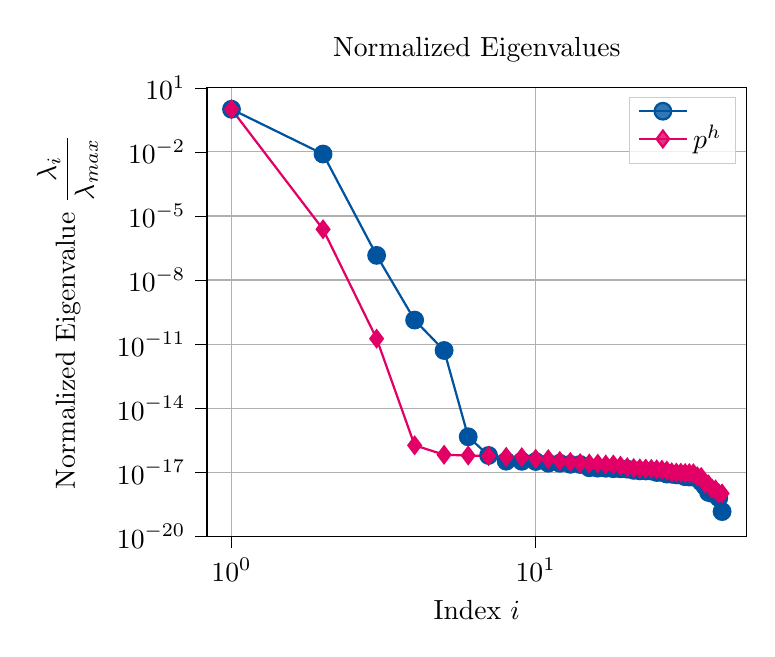
\begin{tikzpicture}

\definecolor{color0}{rgb}{0,0.329411764705882,0.623529411764706}
\definecolor{color1}{rgb}{0.890196078431372,0,0.4}

\begin{axis}[
legend cell align={left},
legend style={fill opacity=0.8, draw opacity=1, text opacity=1, draw=white!80!black},
log basis x={10},
log basis y={10},
tick align=outside,
tick pos=left,
title={Normalized Eigenvalues},
x grid style={white!69.0196078431373!black},
xlabel={Index \(\displaystyle i\)},
xmajorgrids,
xmin=0.830540485032707, xmax=49.3654442364545,
xmode=log,
xtick style={color=black},
xtick={0.01,0.1,1,10,100,1000},
xticklabels={
  \(\displaystyle 10^{-2}\),
  \(\displaystyle 10^{-1}\),
  \(\displaystyle 10^{0}\),
  \(\displaystyle 10^{1}\),
  \(\displaystyle 10^{2}\),
  \(\displaystyle 10^{3}\)
},
y grid style={white!69.0196078431373!black},
ylabel={Normalized Eigenvalue \(\displaystyle \frac{\lambda_i}{\lambda_{\text{max}}}\)},
ymajorgrids,
ymin=1e-20, ymax=10,
ymode=log,
ytick style={color=black},
ytick={1e-23,1e-20,1e-17,1e-14,1e-11,1e-08,1e-05,0.01,10,10000},
yticklabels={
  \(\displaystyle 10^{-23}\),
  \(\displaystyle 10^{-20}\),
  \(\displaystyle 10^{-17}\),
  \(\displaystyle 10^{-14}\),
  \(\displaystyle 10^{-11}\),
  \(\displaystyle 10^{-8}\),
  \(\displaystyle 10^{-5}\),
  \(\displaystyle 10^{-2}\),
  \(\displaystyle 10^{1}\),
  \(\displaystyle 10^{4}\)
}
]
\addplot [thick, color0, mark=*, mark size=3, mark options={solid}]
table {%
1 1
2 0.00794975858415845
3 1.42582257382325e-07
4 1.32791974403868e-10
5 5.00366283890635e-12
6 4.54114155240754e-16
7 6.04573529497411e-17
8 3.26201133022688e-17
9 3.22574638852698e-17
10 3.15358446366046e-17
11 2.62454621731955e-17
12 2.60840954654917e-17
13 2.33242093571454e-17
14 2.28813585566599e-17
15 1.60218882337199e-17
16 1.54306862706516e-17
17 1.52807821353466e-17
18 1.44864745846082e-17
19 1.43851705211444e-17
20 1.38677194525787e-17
21 1.21734236816605e-17
22 1.14897279038485e-17
23 1.13956935268721e-17
24 1.12564920102658e-17
25 9.63808041350083e-18
26 9.58979066065725e-18
27 8.13046505587439e-18
28 8.00740202533402e-18
29 7.46188080562777e-18
30 7.26718042554605e-18
31 6.11314351785897e-18
32 5.93273799548898e-18
33 5.84970067761768e-18
34 5.29939613242502e-18
35 3.47549460184894e-18
36 2.1905261247255e-18
37 1.12228744856004e-18
38 1.01406198292573e-18
39 9.59373162820783e-19
40 6.26226288149959e-19
41 1.42523827201686e-19
};
\addlegendentry{$\trialVelocityHomDiscrete$}
\addplot [thick, color1, mark=diamond*, mark size=3, mark options={solid}]
table {%
1 1
2 2.37328846603967e-06
3 1.78817929292869e-11
4 1.81154657334976e-16
5 6.51678466039161e-17
6 6.02235881107004e-17
7 5.69247083103718e-17
8 5.20065737906182e-17
9 5.01348143603465e-17
10 4.20958043774671e-17
11 4.07622974109276e-17
12 3.32697934377648e-17
13 2.98511733192585e-17
14 2.64421964531683e-17
15 2.52583071694472e-17
16 2.48386648445979e-17
17 2.27569426656641e-17
18 2.27247846357554e-17
19 1.99821382141988e-17
20 1.70491132142761e-17
21 1.54624364513944e-17
22 1.49112670601225e-17
23 1.45406520529215e-17
24 1.40935012359226e-17
25 1.35426769923973e-17
26 1.2976308799412e-17
27 1.18179500955933e-17
28 9.80114361457536e-18
29 9.51423374282225e-18
30 9.36239599182889e-18
31 9.08584610553105e-18
32 8.96571848518543e-18
33 8.78366822577326e-18
34 6.40001828288954e-18
35 5.93546015704658e-18
36 2.97856912325833e-18
37 2.64216217074413e-18
38 1.67829393129063e-18
39 1.53977850304594e-18
40 1.02797999983454e-18
41 1.00473640799576e-18
};
\addlegendentry{$p^h$}
\end{axis}

\end{tikzpicture}

        }
    }
    \subcaptionbox{Maximum interpolation error during the \gls{eim}.\label{fig:valve-likeEIMErrors}}{
        \resizebox{0.44\textwidth}{!}{
        % This file was created by tikzplotlib v0.9.8.
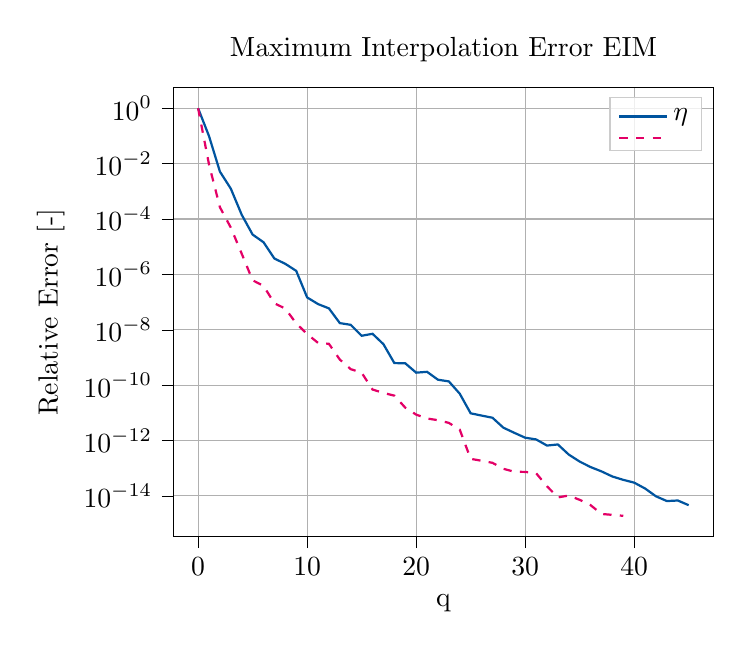
\begin{tikzpicture}

%\definecolor{color0}{rgb}{0.12156862745098,0.466666666666667,0.705882352941177}
%\definecolor{color1}{rgb}{1,0.498039215686275,0.0549019607843137}

\definecolor{color0}{rgb}{0,0.329411764705882,0.623529411764706}
\definecolor{color1}{rgb}{0.890196078431372,0,0.4}

\begin{axis}[
legend cell align={left},
legend style={fill opacity=0.8, draw opacity=1, text opacity=1, draw=white!80!black},
log basis y={10},
tick align=outside,
tick pos=left,
title={Maximum Interpolation Error EIM},
x grid style={white!69.0196078431373!black},
xlabel={q},
xmajorgrids,
xmin=-2.25, xmax=47.25,
xtick style={color=black},
xtick={-10,0,10,20,30,40,50},
xticklabels={
  \(\displaystyle -10\),
  \(\displaystyle 0\),
  \(\displaystyle 10\),
  \(\displaystyle 20\),
  \(\displaystyle 30\),
  \(\displaystyle 40\),
  \(\displaystyle 50\)
},
y grid style={white!69.0196078431373!black},
ylabel={Relative Error [-]},
ymajorgrids,
ymin=3.51471410776371e-16, ymax=5.44389825525944,
ymode=log,
ytick style={color=black},
ytick={1e-18,1e-16,1e-14,1e-12,1e-10,1e-08,1e-06,0.0001,0.01,1,100,10000},
yticklabels={
  \(\displaystyle 10^{-18}\),
  \(\displaystyle 10^{-16}\),
  \(\displaystyle 10^{-14}\),
  \(\displaystyle 10^{-12}\),
  \(\displaystyle 10^{-10}\),
  \(\displaystyle 10^{-8}\),
  \(\displaystyle 10^{-6}\),
  \(\displaystyle 10^{-4}\),
  \(\displaystyle 10^{-2}\),
  \(\displaystyle 10^{0}\),
  \(\displaystyle 10^{2}\),
  \(\displaystyle 10^{4}\)
}
]
\addplot [thick, color0]
table {%
0 1
1 0.0987673453717658
2 0.00515599137631726
3 0.00124900271315819
4 0.000142463479281955
5 2.74366574975223e-05
6 1.44975700969233e-05
7 3.73748485858245e-06
8 2.40757494835904e-06
9 1.34040458242958e-06
10 1.47604939852668e-07
11 8.49109837914781e-08
12 5.91845957000327e-08
13 1.74224683009756e-08
14 1.51054092822489e-08
15 6.07435279360086e-09
16 7.16579464736882e-09
17 3.01910092646183e-09
18 6.27830508569281e-10
19 6.15982655829241e-10
20 2.83140648375761e-10
21 3.03192480175683e-10
22 1.57506587196689e-10
23 1.36631157416829e-10
24 4.91399776836732e-11
25 9.63959118288821e-12
26 7.98281605427662e-12
27 6.6676277667823e-12
28 2.91438313811172e-12
29 1.90614931246576e-12
30 1.26634505351022e-12
31 1.10023595172808e-12
32 6.60646845871169e-13
33 7.2149035717033e-13
34 3.11375616648648e-13
35 1.74109286658845e-13
36 1.10318338826161e-13
37 7.70544122335398e-14
38 5.03169522508634e-14
39 3.8106143754838e-14
40 3.02112244686146e-14
41 1.85267439250041e-14
42 9.68443432443396e-15
43 6.52646660994462e-15
44 6.84226338139356e-15
45 4.63168598125102e-15
};
\addlegendentry{$\eta$}
\addplot [thick, dashed, color1]
table {%
0 1
1 0.00932238039336628
2 0.000266943760459508
3 4.90949857038112e-05
4 5.599960695831e-06
5 6.12824410476193e-07
6 3.86211523959076e-07
7 9.04010167944746e-08
8 5.82744632540993e-08
9 1.70168470184833e-08
10 7.04436726456646e-09
11 3.36213438130085e-09
12 3.11207201674506e-09
13 8.38932040992142e-10
14 3.78263928821779e-10
15 2.82163428907021e-10
16 6.95533441664873e-11
17 5.24268227949716e-11
18 4.19121093616782e-11
19 1.54370265480439e-11
20 8.64749152149743e-12
21 6.24447738563931e-12
22 5.44681941832098e-12
23 4.3396799607452e-12
24 2.47660431675892e-12
25 2.18757513175438e-13
26 1.86329799904232e-13
27 1.57026268596924e-13
28 9.55790405605825e-14
29 7.48084623843346e-14
30 7.36848530815293e-14
31 6.64897673464922e-14
32 2.24123930998593e-14
33 8.85932301724094e-15
34 1.03441814307043e-14
35 7.2349477058683e-15
36 4.64890234819224e-15
37 2.2322703665489e-15
38 2.07282248322398e-15
39 1.91337459989906e-15
};
\addlegendentry{$\tMomPlain$}
\end{axis}

\end{tikzpicture}

        }
    }
    \caption{Valve-like test case: results from the construction of the \gls{rom}.}
    \label{fig:valve-likeOffline}
\end{figure}
\bigskip
\par
To quantify the quality of the \gls{rom}, we perform an error and performance analysis. To that end, we create $\nTest = 50$ testing samples drawn from a uniform distribution. For each sample, we compare the solutions from the \gls{fom} and the \gls{rom} as well as the respective runtimes.
To evaluate the accuracy of the \gls{rom}, we use the following error definitions:
\begin{align}
    \relErrorVelocity
    =
    \frac
    {|\trialVelocityDiscrete-\trialVelocityReduced|_{\sobolevSpaceVector}}
    {|\trialVelocityDiscrete|_{\sobolevSpaceVector}},
    \,
    \relErrorPressure
    =
    \frac
    {||\trialPressureDiscrete-\trialPressureReduced||_{L^2}}
    {||\trialPressureDiscrete||_{L^2}},
\end{align}
where $|\cdot|_{\sobolevSpaceVector}$ and $||\cdot||_{L^2}$ are discrete measures for the $\sobolevSpaceVector$ semi-norm and the $L^2$ norm, respectively. The maximal error over all testing samples is shown in \Cref{fig:valveRelativeErrorMax}, using different numbers of basis functions for the velocity and the pressure field. Note that we ignore the lifting function in these plots, since it does not represent a solution, but is only intended to ensure the Dirichlet boundary conditions.
For the velocity, the error ranges from values smaller than \SI{1e-2}{} to values smaller than \SI{1e-6}{} when increasing the number of basis functions. Similarly, the maximum error in the pressure is limited by \SI{1e-2}{} and drops below \SI{1e-7}{} for $\nBasisVelocityROM$ and $\nBasisPressureROM$ large enough. These results suggest that the error introduced by the \gls{rom} is in a reasonable range for typical engineering applications and, furthermore, that it can be controlled by choosing the number of basis functions such that a desired accuracy is achieved.
\begin{figure}
    \captionsetup[sub]{position=bottom}
    \centering
    \Large
    \subcaptionbox{Velocity.}{
        \resizebox{0.44\textwidth}{!}{
        % This file was created by tikzplotlib v0.9.8.
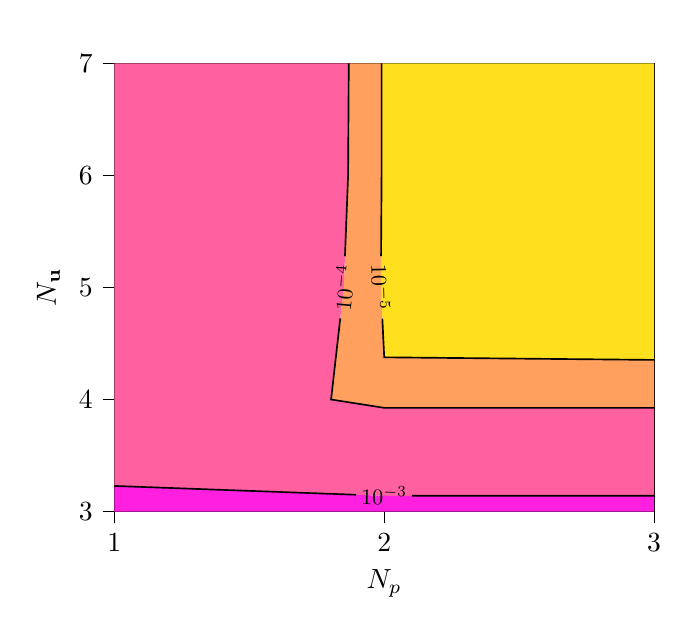
\begin{tikzpicture}

\definecolor{color0}{rgb}{1,0.87843137254902,0.12156862745098}
\definecolor{color1}{rgb}{1,0.627450980392157,0.372549019607843}
\definecolor{color2}{rgb}{1,0.376470588235294,0.623529411764706}
\definecolor{color3}{rgb}{1,0.125490196078431,0.874509803921569}

\begin{axis}[
tick align=outside,
tick pos=left,
%title={Relative Error in Velocity \(\displaystyle \mathbf{u}\) - Max},
title={$\relErrorVelocity$},
x grid style={white!69.0196078431373!black},
xlabel={\(\displaystyle N_p\)},
xmin=1, xmax=3,
xtick style={color=black},
xtick={1,2,3},
xticklabels={\(\displaystyle 1\),\(\displaystyle 2\),\(\displaystyle 3\)},
y grid style={white!69.0196078431373!black},
ylabel={\(\displaystyle N_{\mathbf{u}}\)},
ymin=3, ymax=7,
ytick style={color=black},
ytick={3,4,5,6,7},
yticklabels={
  \(\displaystyle 3\),
  \(\displaystyle 4\),
  \(\displaystyle 5\),
  \(\displaystyle 6\),
  \(\displaystyle 7\)
}
]
\addplot [draw=none, fill=color0]
table{%
x  y
2 4.37650891394412
3 4.35330770412385
3 5
3 6
3 7
2 7
1.99040991259345 7
1.9903127173998 6
1.98760845108052 5
2 4.37650891394412
};
\addplot [draw=none, fill=color1]
table{%
x  y
2 3.92579367910137
3 3.92540471448223
3 4
3 4.35330770412385
2 4.37650891394412
1.98760845108052 5
1.9903127173998 6
1.99040991259345 7
1.86869012295147 7
1.86619036626405 6
1.85013870710813 5
1.80309130655496 4
2 3.92579367910137
};
\addplot [draw=none, fill=color2]
table{%
x  y
2 3.14101234840689
3 3.14081265825156
3 3.92540471448223
2 3.92579367910137
1.80309130655496 4
1.85013870710813 5
1.86619036626405 6
1.86869012295147 7
1 7
1 6
1 5
1 4
1 3.22895886838152
2 3.14101234840689
};
\addplot [draw=none, fill=color3]
table{%
x  y
2 3
3 3
3 3.14081265825156
2 3.14101234840689
1 3.22895886838152
1 3
2 3
};
\path [draw=black, semithick]
(axis cs:3,4.35330770412385)
--(axis cs:2,4.37650891394412)
--(axis cs:1.99313704618645,4.72182414084339);

\path [draw=black, semithick]
(axis cs:1.98836176234379,5.27856400751013)
--(axis cs:1.9903127173998,6)
--(axis cs:1.99040991259345,7);

\path [draw=black, semithick]
(axis cs:3,3.92540471448223)
--(axis cs:2,3.92579367910137)
--(axis cs:1.80309130655496,4)
--(axis cs:1.83713590577805,4.72362338456115);

\path [draw=black, semithick]
(axis cs:1.85460609537104,5.27831317744237)
--(axis cs:1.86619036626405,6)
--(axis cs:1.86869012295147,7);

\path [draw=black, semithick]
(axis cs:3,3.14081265825156)
--(axis cs:2.10379029115697,3.14099162250753);

\path [draw=black, semithick]
(axis cs:1.89626538289669,3.15013544698203)
--(axis cs:1,3.22895886838152);

\draw (axis cs:1.98760845108052,5) node[
  scale=0.8,
  text=black,
  rotate=271.3
]{$10^{-5}$};
\draw (axis cs:1.85013870710813,5) node[
  scale=0.8,
  text=black,
  rotate=85.2
]{$10^{-4}$};
\draw (axis cs:2,3.14101234840689) node[
  scale=0.8,
  text=black,
  rotate=359.1
]{$10^{-3}$};
\end{axis}

\end{tikzpicture}
}
    }
    \subcaptionbox{Pressure.}{
        \resizebox{0.44\textwidth}{!}{
        % This file was created by tikzplotlib v0.9.8.
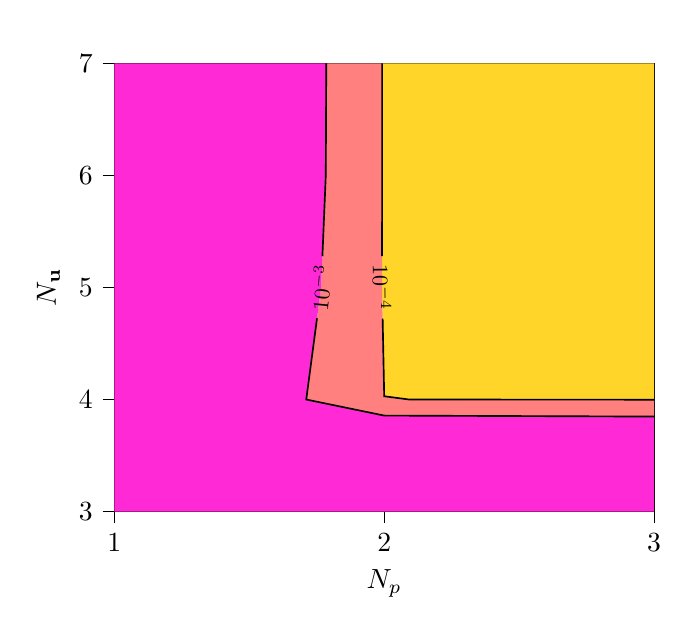
\begin{tikzpicture}

\definecolor{color0}{rgb}{1,0.835294117647059,0.164705882352941}
\definecolor{color1}{rgb}{1,0.501960784313725,0.498039215686275}
\definecolor{color2}{rgb}{1,0.164705882352941,0.835294117647059}

\begin{axis}[
tick align=outside,
tick pos=left,
%title={Relative Error in Pressure \(\displaystyle p\) - Max},
title={$\relErrorPressure$},
x grid style={white!69.0196078431373!black},
xlabel={\(\displaystyle N_p\)},
xmin=1, xmax=3,
xtick style={color=black},
xtick={1,2,3},
xticklabels={\(\displaystyle 1\),\(\displaystyle 2\),\(\displaystyle 3\)},
y grid style={white!69.0196078431373!black},
ylabel={\(\displaystyle N_{\mathbf{u}}\)},
ymin=3, ymax=7,
ytick style={color=black},
ytick={3,4,5,6,7},
yticklabels={
  \(\displaystyle 3\),
  \(\displaystyle 4\),
  \(\displaystyle 5\),
  \(\displaystyle 6\),
  \(\displaystyle 7\)
}
]
\addplot [draw=none, fill=color0]
table{%
x  y
3 3.99841272096808
3 4
3 5
3 6
3 7
2 7
1.99231388686608 7
1.9923086500537 6
1.99186016592534 5
2 4.02906689026844
2.0929081054864 4
3 3.99841272096808
};
\addplot [draw=none, fill=color1]
table{%
x  y
2 3.85666988114318
3 3.84783564712328
3 3.99841272096808
2.0929081054864 4
2 4.02906689026844
1.99186016592534 5
1.9923086500537 6
1.99231388686608 7
1.78528526361933 7
1.78346767600251 6
1.76616198020346 5
1.71107969290604 4
2 3.85666988114318
};
\addplot [draw=none, fill=color2]
table{%
x  y
2 3
3 3
3 3.84783564712328
2 3.85666988114318
1.71107969290604 4
1.76616198020346 5
1.78346767600251 6
1.78528526361933 7
1 7
1 6
1 5
1 4
1 3
2 3
};
\path [draw=black, semithick]
(axis cs:3,3.99841272096808)
--(axis cs:2.0929081054864,4)
--(axis cs:2,4.02906689026844)
--(axis cs:1.99419498249751,4.72149914921187);

\path [draw=black, semithick]
(axis cs:1.99198510066168,5.278571143184)
--(axis cs:1.9923086500537,6)
--(axis cs:1.99231388686608,7);

\path [draw=black, semithick]
(axis cs:3,3.84783564712328)
--(axis cs:2,3.85666988114318)
--(axis cs:1.71107969290604,4)
--(axis cs:1.75098262156661,4.72442395946829);

\path [draw=black, semithick]
(axis cs:1.77097765920204,5.27827133069329)
--(axis cs:1.78346767600251,6)
--(axis cs:1.78528526361933,7);

\draw (axis cs:1.99186016592534,5) node[
  scale=0.8,
  text=black,
  rotate=270.6
]{$10^{-4}$};
\draw (axis cs:1.76616198020346,5) node[
  scale=0.8,
  text=black,
  rotate=84.5
]{$10^{-3}$};
\end{axis}

\end{tikzpicture}
}
    }
    \caption{Valve-like test case: maximum relative error of the \gls{rom} over all testing samples.}
    \label{fig:valveRelativeErrorMax}
\end{figure}
\par
Finally, we investigate the performance of the \gls{rom} by comparing the CPU time needed for a single evaluation of the \gls{rom} to that for the \gls{fom}. Note that the former has been run on a single core, whereas the latter used 64 cores. Also in this analysis, we skip the lifting function for the same reason as before. \Cref{fig:valvePerformance} presents the speed up, i.e., the ratio between the CPU time of \gls{fom} and \gls{rom} evaluations, for different number of basis functions $\nBasisVelocityROM$ and $\nBasisPressureROM$.  Both, the average and the maximum speed up, are in the order of 1000 and indicate that a significant reduction of the runtime for the \gls{rom} is realized. 
\begin{figure}
    \captionsetup[sub]{position=bottom}
    \centering
    \Large
    \subcaptionbox{Average speed up over all testing samples.}{
        \resizebox{0.44\textwidth}{!}{
        % This file was created by tikzplotlib v0.9.8.
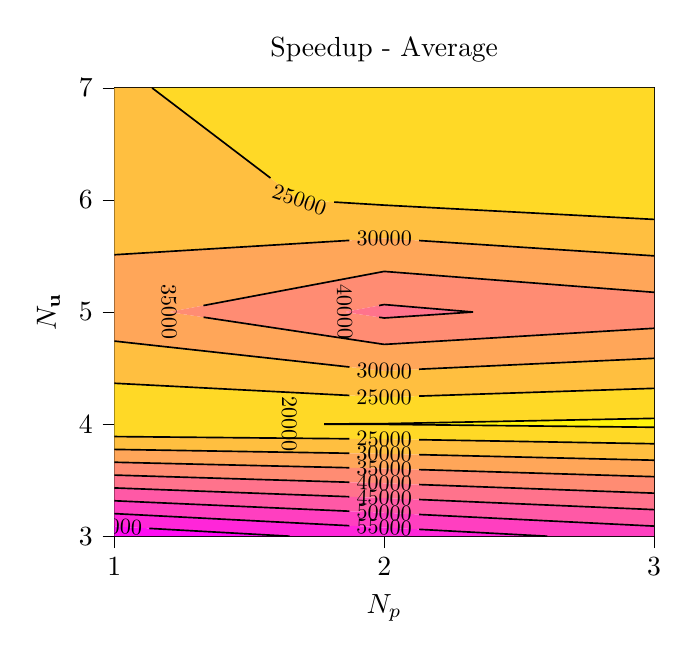
\begin{tikzpicture}

\definecolor{color0}{rgb}{1,0.952941176470588,0.0470588235294118}
\definecolor{color1}{rgb}{1,0.850980392156863,0.149019607843137}
\definecolor{color2}{rgb}{1,0.749019607843137,0.250980392156863}
\definecolor{color3}{rgb}{1,0.650980392156863,0.349019607843137}
\definecolor{color4}{rgb}{1,0.549019607843137,0.450980392156863}
\definecolor{color5}{rgb}{1,0.450980392156863,0.549019607843137}
\definecolor{color6}{rgb}{1,0.349019607843137,0.650980392156863}
\definecolor{color7}{rgb}{1,0.247058823529412,0.752941176470588}
\definecolor{color8}{rgb}{1,0.149019607843137,0.850980392156863}
\definecolor{color9}{rgb}{1,0.0470588235294118,0.952941176470588}

\begin{axis}[
tick align=outside,
tick pos=left,
title={Speedup - Average},
x grid style={white!69.0196078431373!black},
xlabel={\(\displaystyle N_p\)},
xmin=1, xmax=3,
xtick style={color=black},
xtick={1,2,3},
xticklabels={\(\displaystyle 1\),\(\displaystyle 2\),\(\displaystyle 3\)},
y grid style={white!69.0196078431373!black},
ylabel={\(\displaystyle N_{\mathbf{u}}\)},
ymin=3, ymax=7,
ytick style={color=black},
ytick={3,4,5,6,7},
yticklabels={
  \(\displaystyle 3\),
  \(\displaystyle 4\),
  \(\displaystyle 5\),
  \(\displaystyle 6\),
  \(\displaystyle 7\)
}
]
\addplot [draw=none, fill=color0]
table{%
x  y
2 3.99776029877739
3 3.97186061500088
3 4
3 4.05129247948725
2 4.00401665310977
1.64783776122399 4
2 3.99776029877739
};
\addplot [draw=none, fill=color1]
table{%
x  y
2 3.86632751738316
3 3.82489079580478
3 3.97186061500088
2 3.99776029877739
1.64783776122399 4
2 4.00401665310977
3 4.05129247948725
3 4.31918911036938
2 4.23972661512697
1 4.36447852644752
1 4
1 3.88899847255399
2 3.86632751738316
};
\addplot [draw=none, fill=color1]
table{%
x  y
2 5.95377752187074
3 5.82647002301902
3 6
3 7
2 7
1.13955470147603 7
1.68538959041588 6
2 5.95377752187074
};
\addplot [draw=none, fill=color2]
table{%
x  y
2 3.73489473598894
3 3.67792097660869
3 3.82489079580478
2 3.86632751738316
1 3.88899847255399
1 3.77440465802077
2 3.73489473598894
};
\addplot [draw=none, fill=color2]
table{%
x  y
2 4.23972661512697
3 4.31918911036938
3 4.58708574125151
2 4.47543657714418
1 4.74075248971692
1 4.36447852644752
2 4.23972661512697
};
\addplot [draw=none, fill=color2]
table{%
x  y
2 5.65807486026756
3 5.50125704822069
3 5.82647002301902
2 5.95377752187074
1.68538959041588 6
1.13955470147603 7
1 7
1 6
1 5.51094647432634
2 5.65807486026756
};
\addplot [draw=none, fill=color3]
table{%
x  y
2 3.60346195459471
3 3.5309511574126
3 3.67792097660869
2 3.73489473598894
1 3.77440465802077
1 3.65981084348756
2 3.60346195459471
};
\addplot [draw=none, fill=color3]
table{%
x  y
2 4.47543657714418
3 4.58708574125151
3 4.85498237213365
2 4.71114653916139
1.20242039825908 5
2 5.36237219866437
3 5.17604407342235
3 5.50125704822069
2 5.65807486026756
1 5.51094647432634
1 5
1 4.74075248971692
2 4.47543657714418
};
\addplot [draw=none, fill=color4]
table{%
x  y
2 3.47202917320049
3 3.38398133821651
3 3.5309511574126
2 3.60346195459471
1 3.65981084348756
1 3.54521702895434
2 3.47202917320049
};
\addplot [draw=none, fill=color4]
table{%
x  y
2 4.71114653916139
3 4.85498237213365
3 5
3 5.17604407342235
2 5.36237219866437
1.20242039825908 5
2 4.71114653916139
1.85326064468108 5
2 5.06666953706118
2.3295534889383 5
2 4.94685650117859
1.85326064468108 5
};
\addplot [draw=none, fill=color5]
table{%
x  y
2 3.34059639180626
3 3.23701151902041
3 3.38398133821651
2 3.47202917320049
1 3.54521702895434
1 3.43062321442112
2 3.34059639180626
};
\addplot [draw=none, fill=color5]
table{%
x  y
2 4.94685650117859
2.3295534889383 5
2 5.06666953706118
1.85326064468108 5
2 4.94685650117859
};
\addplot [draw=none, fill=color6]
table{%
x  y
2 3.20916361041203
3 3.09004169982432
3 3.23701151902041
2 3.34059639180626
1 3.43062321442112
1 3.3160293998879
2 3.20916361041203
};
\addplot [draw=none, fill=color7]
table{%
x  y
2 3.07773082901781
2.60424735056556 3
3 3
3 3.09004169982432
2 3.20916361041203
1 3.3160293998879
1 3.20143558535469
2 3.07773082901781
};
\addplot [draw=none, fill=color8]
table{%
x  y
2 3
2.60424735056556 3
2 3.07773082901781
1 3.20143558535469
1 3.08684177082147
1.64970439596316 3
2 3
};
\addplot [draw=none, fill=color9]
table{%
x  y
1 3.08684177082147
1 3
1.64970439596316 3
1 3.08684177082147
};
\path [draw=black, semithick]
(axis cs:3,3.97186061500088)
--(axis cs:2,3.99776029877739)
--(axis cs:1.77726149904818,3.99917688362941);

\path [draw=black, semithick]
(axis cs:1.77726069380053,4.00147615776869)
--(axis cs:2,4.00401665310977)
--(axis cs:3,4.05129247948725);

\path [draw=black, semithick]
(axis cs:3,3.82489079580478)
--(axis cs:2.12940867994302,3.86096524594254);

\path [draw=black, semithick]
(axis cs:1.87058051564284,3.86926158071125)
--(axis cs:1,3.88899847255399);

\path [draw=black, semithick]
(axis cs:1,4.36447852644752)
--(axis cs:1.87071547689406,4.2558551064886);

\path [draw=black, semithick]
(axis cs:2.12936741661236,4.25000647285406)
--(axis cs:3,4.31918911036938);

\path [draw=black, semithick]
(axis cs:3,5.82647002301902)
--(axis cs:2,5.95377752187074)
--(axis cs:1.81462022259509,5.98101346971504);

\path [draw=black, semithick]
(axis cs:1.57849420274952,6.1958383200348)
--(axis cs:1.13955470147603,7);

\path [draw=black, semithick]
(axis cs:3,3.67792097660869)
--(axis cs:2.1293949518265,3.72752261913855);

\path [draw=black, semithick]
(axis cs:1.87058991946085,3.74000771818117)
--(axis cs:1,3.77440465802077);

\path [draw=black, semithick]
(axis cs:1,4.74075248971692)
--(axis cs:1.87120364443596,4.5096082997567);

\path [draw=black, semithick]
(axis cs:2.12931226725914,4.48987418369249)
--(axis cs:3,4.58708574125151);

\path [draw=black, semithick]
(axis cs:3,5.50125704822069)
--(axis cs:2.12920375458042,5.63781341016601);

\path [draw=black, semithick]
(axis cs:1.87076991649158,5.63906144666591)
--(axis cs:1,5.51094647432634);

\path [draw=black, semithick]
(axis cs:3,3.5309511574126)
--(axis cs:2.12937689557672,3.5940807327595);

\path [draw=black, semithick]
(axis cs:1.87060441248816,3.61075325217864)
--(axis cs:1,3.65981084348756);

\path [draw=black, semithick]
(axis cs:3,5.17604407342235)
--(axis cs:2,5.36237219866437)
--(axis cs:1.33002909148532,5.05797771486651);

\path [draw=black, semithick]
(axis cs:1.33068211116719,4.95354841123603)
--(axis cs:2,4.71114653916139)
--(axis cs:3,4.85498237213365);

\path [draw=black, semithick]
(axis cs:3,3.38398133821651)
--(axis cs:2.12935451663035,3.46063978806578);

\path [draw=black, semithick]
(axis cs:1.87062398959549,3.48149792598798)
--(axis cs:1,3.54521702895434);

\path [draw=black, semithick]
(axis cs:1.98152235758919,4.95354841123603)
--(axis cs:2,4.94685650117859)
--(axis cs:2.3295534889383,5)
--(axis cs:2,5.06666953706118)
--(axis cs:1.98086933790731,5.05797771486651);

\path [draw=black, semithick]
(axis cs:3,3.23701151902041)
--(axis cs:2.12932782172,3.32719998584572);

\path [draw=black, semithick]
(axis cs:1.87064864385909,3.35224148340055)
--(axis cs:1,3.43062321442112);

\path [draw=black, semithick]
(axis cs:3,3.09004169982432)
--(axis cs:2.12929681886861,3.19376152631549);

\path [draw=black, semithick]
(axis cs:1.87067836656755,3.2229836688651)
--(axis cs:1,3.3160293998879);

\path [draw=black, semithick]
(axis cs:2.60424735056556,3)
--(axis cs:2.12927570066499,3.06110070664302);

\path [draw=black, semithick]
(axis cs:1.87071314723031,3.09372422763725)
--(axis cs:1,3.20143558535469);

\path [draw=black, semithick]
(axis cs:1.64970439596316,3)
--(axis cs:1.12926390778472,3.06956390303255);

\draw (axis cs:1.64783776122399,4) node[
  scale=0.8,
  text=black,
  rotate=270.1
]{20000};
\draw (axis cs:2,3.86632751738316) node[
  scale=0.8,
  text=black,
  rotate=359.3
]{25000};
\draw (axis cs:2,4.23972661512697) node[
  scale=0.8,
  text=black,
  rotate=359.5
]{25000};
\draw (axis cs:1.68538959041588,6) node[
  scale=0.8,
  text=black,
  rotate=341.3
]{25000};
\draw (axis cs:2,3.73489473598894) node[
  scale=0.8,
  text=black,
  rotate=359.0
]{30000};
\draw (axis cs:2,4.47543657714418) node[
  scale=0.8,
  text=black,
  rotate=358.4
]{30000};
\draw (axis cs:2,5.65807486026756) node[
  scale=0.8,
  text=black,
  rotate=359.9
]{30000};
\draw (axis cs:2,3.60346195459471) node[
  scale=0.8,
  text=black,
  rotate=358.6
]{35000};
\draw (axis cs:1.20242039825908,5) node[
  scale=0.8,
  text=black,
  rotate=271.0
]{35000};
\draw (axis cs:2,3.47202917320049) node[
  scale=0.8,
  text=black,
  rotate=358.3
]{40000};
\draw (axis cs:1.85326064468108,5) node[
  scale=0.8,
  text=black,
  rotate=271.0
]{40000};
\draw (axis cs:2,3.34059639180626) node[
  scale=0.8,
  text=black,
  rotate=357.9
]{45000};
\draw (axis cs:2,3.20916361041203) node[
  scale=0.8,
  text=black,
  rotate=357.6
]{50000};
\draw (axis cs:2,3.07773082901781) node[
  scale=0.8,
  text=black,
  rotate=357.3
]{55000};
\draw (axis cs:1,3.08684177082147) node[
  scale=0.8,
  text=black,
  rotate=357.1
]{60000};
\end{axis}

\end{tikzpicture}
}
    }
    \subcaptionbox{Maximum speed up over all testing samples.}{
        \resizebox{0.44\textwidth}{!}{
        % This file was created by tikzplotlib v0.9.8.
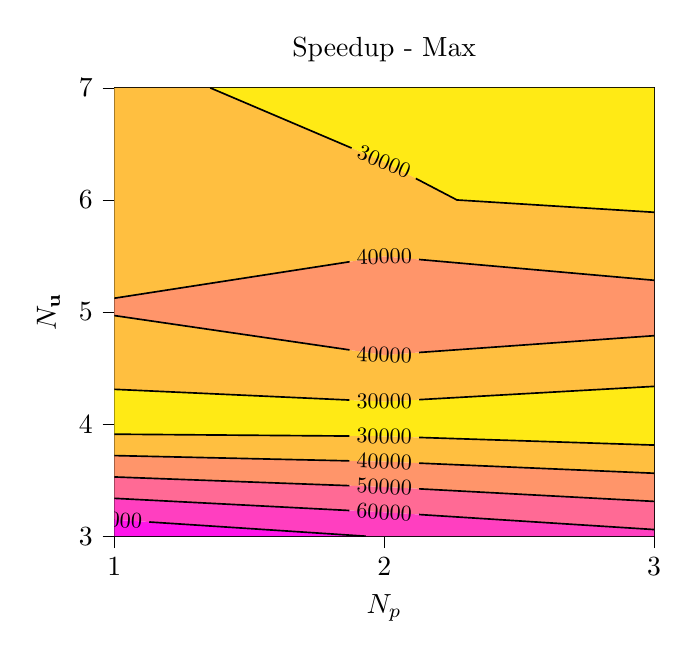
\begin{tikzpicture}

\definecolor{color0}{rgb}{1,0.917647058823529,0.0823529411764706}
\definecolor{color1}{rgb}{1,0.749019607843137,0.250980392156863}
\definecolor{color2}{rgb}{1,0.584313725490196,0.415686274509804}
\definecolor{color3}{rgb}{1,0.415686274509804,0.584313725490196}
\definecolor{color4}{rgb}{1,0.247058823529412,0.752941176470588}
\definecolor{color5}{rgb}{1,0.0823529411764706,0.917647058823529}

\begin{axis}[
tick align=outside,
tick pos=left,
title={Speedup - Max},
x grid style={white!69.0196078431373!black},
xlabel={\(\displaystyle N_p\)},
xmin=1, xmax=3,
xtick style={color=black},
xtick={1,2,3},
xticklabels={\(\displaystyle 1\),\(\displaystyle 2\),\(\displaystyle 3\)},
y grid style={white!69.0196078431373!black},
ylabel={\(\displaystyle N_{\mathbf{u}}\)},
ymin=3, ymax=7,
ytick style={color=black},
ytick={3,4,5,6,7},
yticklabels={
  \(\displaystyle 3\),
  \(\displaystyle 4\),
  \(\displaystyle 5\),
  \(\displaystyle 6\),
  \(\displaystyle 7\)
}
]
\addplot [draw=none, fill=color0]
table{%
x  y
2 3.89113969366561
3 3.81295761379902
3 4
3 4.33664393194555
2 4.20059943824401
1 4.31046717020061
1 4
1 3.91000519290614
2 3.89113969366561
};
\addplot [draw=none, fill=color0]
table{%
x  y
3 5.8901285826523
3 6
3 7
2 7
1.35534430289395 7
2 6.33923453361608
2.26948248989546 6
3 5.8901285826523
};
\addplot [draw=none, fill=color1]
table{%
x  y
2 3.66515692779255
3 3.56174755756104
3 3.81295761379902
2 3.89113969366561
1 3.91000519290614
1 3.71929144543007
2 3.66515692779255
};
\addplot [draw=none, fill=color1]
table{%
x  y
2 4.20059943824401
3 4.33664393194555
3 4.78877856727545
2 4.61702317811216
1 4.96839799320352
1 4.31046717020061
2 4.20059943824401
};
\addplot [draw=none, fill=color1]
table{%
x  y
2 5.49635319629926
3 5.28342883044444
3 5.8901285826523
2.26948248989546 6
2 6.33923453361608
1.35534430289395 7
1 7
1 6
1 5.12326574274158
2 5.49635319629926
};
\addplot [draw=none, fill=color2]
table{%
x  y
2 3.4391741619195
3 3.31053750132306
3 3.56174755756104
2 3.66515692779255
1 3.71929144543007
1 3.52857769795399
2 3.4391741619195
};
\addplot [draw=none, fill=color2]
table{%
x  y
2 4.61702317811216
3 4.78877856727545
3 5
3 5.28342883044444
2 5.49635319629926
1 5.12326574274158
1 5
1 4.96839799320352
2 4.61702317811216
};
\addplot [draw=none, fill=color3]
table{%
x  y
2 3.21319139604645
3 3.05932744508508
3 3.31053750132306
2 3.4391741619195
1 3.52857769795399
1 3.33786395047791
2 3.21319139604645
};
\addplot [draw=none, fill=color4]
table{%
x  y
2 3
3 3
3 3.05932744508508
2 3.21319139604645
1 3.33786395047791
1 3.14715020300184
1.93165335182826 3
2 3
};
\addplot [draw=none, fill=color5]
table{%
x  y
1 3.14715020300184
1 3
1.93165335182826 3
1 3.14715020300184
};
\path [draw=black, semithick]
(axis cs:3,3.81295761379902)
--(axis cs:2.12936922751048,3.8810253383881);

\path [draw=black, semithick]
(axis cs:1.87057909585802,3.89358128363441)
--(axis cs:1,3.91000519290614);

\path [draw=black, semithick]
(axis cs:1,4.31046717020061)
--(axis cs:1.87068419689434,4.21480707223737);

\path [draw=black, semithick]
(axis cs:2.12925816089073,4.21818429929918)
--(axis cs:3,4.33664393194555);

\path [draw=black, semithick]
(axis cs:3,5.8901285826523)
--(axis cs:2.26948248989546,6)
--(axis cs:2.11717612375158,6.19172889157148);

\path [draw=black, semithick]
(axis cs:1.87909257266006,6.46316340444465)
--(axis cs:1.35534430289395,7);

\path [draw=black, semithick]
(axis cs:3,3.56174755756104)
--(axis cs:2.12932814733133,3.65178318552381);

\path [draw=black, semithick]
(axis cs:1.87060221616005,3.67216181440409)
--(axis cs:1,3.71929144543007);

\path [draw=black, semithick]
(axis cs:1,4.96839799320352)
--(axis cs:1.87167093357662,4.66211478009752);

\path [draw=black, semithick]
(axis cs:2.12915991192253,4.63920708904871)
--(axis cs:3,4.78877856727545);

\path [draw=black, semithick]
(axis cs:3,5.28342883044444)
--(axis cs:2.12901874905936,5.46888196097241);

\path [draw=black, semithick]
(axis cs:1.87180845969371,5.44852654095875)
--(axis cs:1,5.12326574274158);

\path [draw=black, semithick]
(axis cs:3,3.31053750132306)
--(axis cs:2.12927571007098,3.42254456627974);

\path [draw=black, semithick]
(axis cs:1.87064764090286,3.45073872021719)
--(axis cs:1,3.52857769795399);

\path [draw=black, semithick]
(axis cs:3,3.05932744508508)
--(axis cs:2.12921195720541,3.19331033379938);

\path [draw=black, semithick]
(axis cs:1.87071529966112,3.22930964988661)
--(axis cs:1,3.33786395047791);

\path [draw=black, semithick]
(axis cs:1.93165335182826,3)
--(axis cs:1.12920058312662,3.12674358717447);

\draw (axis cs:2,3.89113969366561) node[
  scale=0.8,
  text=black,
  rotate=359.0
]{30000};
\draw (axis cs:2,4.20059943824401) node[
  scale=0.8,
  text=black,
  rotate=0.3
]{30000};
\draw (axis cs:2,6.33923453361608) node[
  scale=0.8,
  text=black,
  rotate=337.0
]{30000};
\draw (axis cs:2,3.66515692779255) node[
  scale=0.8,
  text=black,
  rotate=358.3
]{40000};
\draw (axis cs:2,4.61702317811216) node[
  scale=0.8,
  text=black,
  rotate=358.1
]{40000};
\draw (axis cs:2,5.49635319629926) node[
  scale=0.8,
  text=black,
  rotate=1.7
]{40000};
\draw (axis cs:2,3.4391741619195) node[
  scale=0.8,
  text=black,
  rotate=357.7
]{50000};
\draw (axis cs:2,3.21319139604645) node[
  scale=0.8,
  text=black,
  rotate=357.0
]{60000};
\draw (axis cs:1,3.14715020300184) node[
  scale=0.8,
  text=black,
  rotate=356.6
]{70000};
\end{axis}

\end{tikzpicture}
}
    }
    \caption{Valve-like test case: performance results.}
    \label{fig:valvePerformance}
\end{figure}
\par
Taken together, the error and performance analysis confirms the effectiveness of the approach for this two-dimensional deforming domain problem with topology changes. In particular, the accuracy of the \gls{rom} is acceptable as well as controllable while a significant reduction of the  computational demands is achieved, too. This qualifies the \gls{rom} as a surrogate model, e.g., in one of the aforementioned many query scenarios.   
\subsection{Artery-Like Geometry with Compression}
After presenting results for a spatially deforming two-dimensional geometry, we will now demonstrate the aptitude of the proposed approach also for the three-dimensional case, resulting in a four-dimensional space-time domain. The geometry is inspired by an artery that locally undergoes compression over time. The initial spatial geometry can be seen in \Cref{fig:arteryGeoInitialFront,fig:arteryGeoInitialSide,fig:arteryGeoInitialTop}. It has a length of $L = \SI{60e-3}{\meter}$ and a radius of $r_0 = \SI{5e-3}{\meter}$.
We are interested in the internal flow over a time period of $\SI{1}{\second}$ where fluid enters on the left-hand side, i.e., at $x_{\text{min}}$ .
The local narrowing of the artery happens according to the following expression for the upper and lower parts of the moving boundary:
\begin{align*}
    y(t) = \pm  \left[ 0.2 + 0.2 \cdot\left(\cos{(\pi\, t\,\si{\per\second})}+1\right)\right] \cdot r_0 .%, \, r_0 = \SI{5e-3}{\meter}. 
\end{align*}
The final state of the deformed spatial geometry is depicted in \Cref{fig:arteryGeoFinalSide,fig:arteryGeoFinalTop}.
\iffalse
Since we assume no-slip conditions along the walls, 
$x \in  [-\SI{30}{\milli\meter}, \SI{30}{\milli\meter}], \,  y \in [-\SI{5}{\milli\meter},\SI{5}{\milli\meter}], \, z \in [-\SI{5}{\milli\meter},\SI{5}{\milli\meter}], \, t \in [ \SI{0}{\second} ,\SI{1}{\second}]$. 
\fi
\par
To mimic blood, the density is set to $\density = \SI{1058}{\kilo\gram\per\cubic\meter}$ and the parameters for the viscosity model are chosen as presented in \cite{Cho1991}:
% etaZero 0.16 etaInf 0.0035 relaxTime 8.2 transRegionExponent 0.64 powerIndex 0.2128
\begin{align*}
    \visc_0 = \SI{0.056}{Pa\cdot s}, \,
    \visc_{\infty} = \SI{0.00345}{Pa\cdot s}, \,
    \lambda = \SI{1.902}{s}, \,
    a = \SI{1.25}{}, \,
    n = \SI{0.22}{}.
\end{align*}
\par
For the inflow velocity, we prescribe the following time-dependent profile:
%1.0e-1*(1-((sqrt(y*y+z*z)/0.005)*(sqrt(y*y+z*z)/0.005)))*(sqrt(t/0.2)*heaviside(0.2-t)+heaviside(t-0.2))
\begin{align*}
    \begin{aligned}
        \velX = \velX_{\text{in}}^0 \lp 1 - \frac{(y^2+z^2)}{r_0^2} \rp  \cdot 
        \begin{cases}  
            \sqrt{\frac{t}{\SI{0.2}{\second}}}    &\text{ for } t < \SI{0.2}{\second},
            \\
            1   &\text{ for } t \ge \SI{0.2}{\second},
        \end{cases}
    \end{aligned}
    \quad
    \begin{aligned}
        \velY = \SI{0}{\meter\per\second}, \quad \velZ = \SI{0}{\meter\per\second},       
    \end{aligned}
    \label{eq:artery-likeInflow}
\end{align*}
with the velocity vector $\trialVelocity = \lb \velX, \velY, \velZ \rb^T$ and $\velX_{\text{in}}^0=\SI{0.1}{\meter\per\second}$. At the outlet, a parallel outflow is enforced, i.e., $\velY=\velZ=0$. Along the walls, no-slip conditions are set. To account for the narrowing, we apply the following boundary conditions for the velocity in $y$-direction on the horizontal and rounded parts:
\begin{align}
   \velY = \frac{\partial y(t)}{\partial t} = \mp \pi \sin(\pi t)\times 10^{-3}\,\si{\meter\per\second}.% = \frac{\pi}{1000} \sin(\pi t) \, \si{\meter\per\second}
\end{align}
The sign of this term depends on whether you consider the upper or the lower part. In particular, the negative and the positive sign correspond to a downward movement for $y>0$ and an upward movement for $y<0$, respectively. 
For this geometry, a locally refined boundary-conforming simplex space-time mesh is constructed using a four-dimensional elastic mesh update~\cite{Danwitz2021}.
\Cref{fig:artery-likeVelocityInitial,fig:artery-likeVelocityFinal} show the resulting velocity field along the artery in its center plane for the initial and final state.
\newcommand{\myW}{0.48\textwidth} 
\begin{figure}
\captionsetup[sub]{position=bottom}
\centering
\subcaptionbox{Front view.\label{fig:arteryGeoInitialFront}}{
 %  \tikzsetnextfilename{topology-arteryFront}
   \begin{tikzpicture}[
    axis/.style={thick, ->},
    every node/.style={color=black}
    ]
       \node at (0,0) [inner sep=0pt, anchor=south west] {\includegraphics[width=\myW,trim={0cm 0cm 0cm 0cm},clip]{fig/artery-like/geometry/frontView/artery-like_3DGeometryFrontView.png}};
       \draw[axis] (0.2*\myW,0.05*\myW)  -- (0.3*\myW,0.05*\myW) node(xline)[right]{$z$};
       \draw[axis] (0.2*\myW,0.05*\myW)  -- (0.2*\myW,0.15*\myW) node(xline)[right]{$y$};
\end{tikzpicture}
}
\subcaptionbox{Side view at $t=0.0\,$s.\label{fig:arteryGeoInitialSide}}{
%\tikzsetnextfilename{topology-arterySide}
\begin{tikzpicture}[
    axis/.style={thick, ->},
    every node/.style={color=black}
    ]
       \node at (0,0) [inner sep=0pt, anchor=south west] {\includegraphics[width=\myW,trim={0cm 20cm 0cm 0cm},clip]{fig/artery-like/geometry/sideView/artery-like_3DSideView.0000.png}};
       \draw[axis] (0.1*\myW,0.05*\myW)  -- (0.2*\myW,0.05*\myW) node(xline)[right]{$x$};
       \draw[axis] (0.1*\myW,0.05*\myW)  -- (0.1*\myW,0.15*\myW) node(xline)[right]{$y$};
\end{tikzpicture}
}\subcaptionbox{Top view $t=0.0\,$s.\label{fig:arteryGeoInitialTop}}{
   %\tikzsetnextfilename{topology-arteryTop}
\begin{tikzpicture}[
    axis/.style={thick, ->},
    every node/.style={color=black}
    ]
       \node at (0,0) [inner sep=0pt, anchor=south west] {\includegraphics[width=\myW,trim={0cm 20cm 0cm 0cm},clip]{
       fig/artery-like/geometry/topView/artery-like_3DGeometryTopView.0000.png}};
       \draw[axis] (0.1*\myW,0.15*\myW)  -- (0.2*\myW,0.15*\myW) node(xline)[right]{$x$};
       \draw[axis] (0.1*\myW,0.15*\myW)  -- (0.1*\myW,0.05*\myW) node(xline)[right]{$z$};
\end{tikzpicture}
}\\
\subcaptionbox{Side view at $t=\SI{1}{\second}$.\label{fig:arteryGeoFinalSide}}{
 %   \tikzsetnextfilename{topology-arteryCSide}
\begin{tikzpicture}[
    axis/.style={thick, ->},
    every node/.style={color=black}
    ]
       \node at (0,0) [inner sep=0pt, anchor=south west] {\includegraphics[width=\myW,trim={0cm 20cm 0cm 0cm},clip]{fig/artery-like/geometry/sideView/artery-like_3DSideView.0034.png}};
       \draw[axis] (0.1*\myW,0.05*\myW)  -- (0.2*\myW,0.05*\myW) node(xline)[right]{$x$};
       \draw[axis] (0.1*\myW,0.05*\myW)  -- (0.1*\myW,0.15*\myW) node(xline)[right]{$y$};
\end{tikzpicture}
}\subcaptionbox{Top view at $t=\SI{1}{\second}$.\label{fig:arteryGeoFinalTop}}{
    % \tikzsetnextfilename{topology-arteryCTop}
 \begin{tikzpicture}[
    axis/.style={thick, ->},
    every node/.style={color=black}
    ]
       \node at (0,0) [inner sep=0pt, anchor=south west] {\includegraphics[width=\myW,trim={0cm 20cm 0cm 0cm},clip]{fig/artery-like/geometry/topView/artery-like_3DGeometryTopView.0034.png}};
       \draw[axis] (0.1*\myW,0.15*\myW)  -- (0.2*\myW,0.15*\myW) node(xline)[right]{$x$};
       \draw[axis] (0.1*\myW,0.15*\myW)  -- (0.1*\myW,0.05*\myW) node(xline)[right]{$z$};
\end{tikzpicture}
}
\caption{Artery-like test case: geometry.}
\label{fig:arteryGeo}
\end{figure}




%%%%%%%%%%%%%%%%%%%%%%%%%% BEGIN HIDDEN
\iffalse
\subsubsection{4D mesh generation}

The space-time finite element simulation of considered transient three-dimensional problem requires a four-dimensional mesh. To generate a four-dimensional pentatope mesh, we follow the procedure outlined in~\cite{danwitz2021four}. In this section, we describe the essential test case specific steps and provide reference with more details on the underlying algorithms.

\renewcommand{\myD}{0.9\textwidth}
\begin{figure}
\centering
% \tikzsetnextfilename{topology-arteryMesh}
\begin{tikzpicture}[
    axis/.style={very thick, ->},
    every node/.style={color=black}
    ]
       \node at (0,0) [inner sep=0pt, anchor=south west] {\includegraphics[width=\myD,trim={0cm 0cm 0cm 0cm},clip]{fig/artery-like/xyt}};
       \draw[axis] (0.014*\myD,0.434*\myD)  -- (0.11*\myD,0.45*\myD) node(xline)[above]{$x$};
       \draw[axis] (0.014*\myD,0.434*\myD)  -- (0.0*\myD,0.5*\myD) node(xline)[right]{$y$};
       \draw[axis] (0.014*\myD,0.434*\myD)  -- (0.016*\myD,0.3*\myD) node(xline)[left]{$t$};
\end{tikzpicture}
\caption{Clamped artery. $x$-$y$-$t$-Mesh.}
\label{fig:arteryMesh}
\end{figure}

Starting point of the pentatope mesh generation for the Artery-like geometry is the tetrahedral mesh shown in Figure~\ref{fig:arteryMesh}. The $x$-$y$-$t$-Mesh can be seen as a space-time mesh for the two-dimensional center plan ($z=0$) of the artery. Please, note that  tetrahedral mesh is refined in the clamp region.

\renewcommand{\myD}{0.9\textwidth}
\begin{figure}
\centering
% \tikzsetnextfilename{topology-arteryMesh}
\begin{tikzpicture}[
    axis/.style={very thick, ->},
    every node/.style={color=black}
    ]
       \node at (0,0) [inner sep=0pt, anchor=south west] {\includegraphics[width=\myD,trim={0cm 0cm 0cm 0cm},clip]{fig/artery-like/Nnt}};
       \draw[axis] (0.014*\myD,0.434*\myD)  -- (0.11*\myD,0.45*\myD) node(xline)[above]{$x$};
       \draw[axis] (0.014*\myD,0.434*\myD)  -- (0.0*\myD,0.5*\myD) node(xline)[right]{$y$};
       \draw[axis] (0.014*\myD,0.434*\myD)  -- (0.016*\myD,0.3*\myD) node(xline)[left]{$t$};
\end{tikzpicture}
\caption{Clamped artery. Nodes inserted during mesh extrusion from 3D to 4D.}
\label{fig:arteryNnt}
\end{figure}

Then, following Behr~\cite{behr2008simplex}, the mesh is extruded in the fourth dimension, nodes are inserted, and a pentatope triangulation is generated. We want to point out that the resulting mesh is refined isotropic in time and all three space directions. The locally refined pentatope mesh is obtained by adjusting the number of nodes inserted to the four-dimensional geometry and the expected flow field. In Figure~\ref{fig:arteryNnt}, the x-y-t-mesh is colored according to the number of nodes inserted in the fourth dimension. The resulting mesh consists of \num{14319807} pentatopes that connect \num{815874} nodes. For further details and application cases with locally refined pentatope meshes, we refer to the descriptions in~\cite{behr2008simplex, karyofylli2018simplex, danwitz2019simplex}.

\renewcommand{\myW}{0.48\textwidth} 
\begin{figure}
\captionsetup[sub]{position=bottom}
\centering
\subcaptionbox{Top view $t=0.0\,$s.}{
   %\tikzsetnextfilename{topology-arteryTop}
\begin{tikzpicture}[
    axis/.style={thick, ->},
    every node/.style={color=black}
    ]
       \node at (0,0) [inner sep=0pt, anchor=south west] {\includegraphics[width=\myW,trim={0cm 0cm 0cm 0cm},clip]{
       fig/artery-like/yzSquare}};
       \draw[axis] (0.1*\myW,0.05*\myW)  -- (0.2*\myW,0.05*\myW) node(xline)[right]{$y$};
       \draw[axis] (0.1*\myW,0.05*\myW)  -- (0.1*\myW,0.15*\myW) node(xline)[right]{$z$};
\end{tikzpicture}
}\subcaptionbox{Side view at $t=0.5\,$s.}{
 %   \tikzsetnextfilename{topology-arteryCSide}
\begin{tikzpicture}[
    axis/.style={thick, ->},
    every node/.style={color=black}
    ]
       \node at (0,0) [inner sep=0pt, anchor=south west] {\includegraphics[width=\myW,trim={0cm 0cm 0cm 0cm},clip]{fig/artery-like/yzCircle}};
       \draw[axis] (0.1*\myW,0.05*\myW)  -- (0.2*\myW,0.05*\myW) node(xline)[right]{$y$};
       \draw[axis] (0.1*\myW,0.05*\myW)  -- (0.1*\myW,0.15*\myW) node(xline)[right]{$z$};
\end{tikzpicture}
}
\caption{Clamped artery. Two representative triangular meshes on the geometry at $x=0$, $t=0$ before and after the application of the elastic mesh update}
\label{fig:arteryxZeroMeshes}
\end{figure}

After extrusion, the mesh cross-section at $x=0$, $t=0$ is a square. To obtain the approximately circular cross-section of the artery-like geometry, we apply an four-dimensional elastic mesh update method (4DEMUM)~\cite{danwitz2021four}. Figure~\ref{fig:arteryxZeroMeshes} visualizes the elastic mesh update with two representative triangular meshes on the geometry.

In the 4DEMUM procedure, the space-time coordinates $[x,y,z,t]^T$ are identified with four spatial coordinates $[x_1, x_2, x_3, x_4]^T$. Following~\cite[Section 4.2.2]{danwitz2021four}, we prescribe the displacements on the pentatope mesh boundary, 
\begin{equation}
 	\label{eq:artDisp}
 	   \mathbf{g}^h =  0.9 \left[  \begin{array}{c}
	     0 \\
	     \left( \sqrt{1-\frac{1}{2} x_3^2 } -1\right) x_2\\ 
	     \left( \sqrt{1-\frac{1}{2} x_2^2} -1\right) x_3\\ 
	     0  \end{array} \right].  \quad
\end{equation}
This boundary condition $\mathbf{g}^h$ maps the square cross-section in the $x_2$-$x_3$-plane onto an approximately circular shape (see Figure~\ref{fig:arteryxZeroMeshes} on the right).

In a final step before the transient simulation, the spatial coordinates $[x_1, x_2, x_3, x_4]^T$ are again identified with the space-time coordinates $[x,y,z,t]^T$ and the mesh is scaled such that $x \in  [-\SI{3}{\centi\meter}, \SI{3}{\centi\meter}], \,  y \in [-\SI{0.5}{\centi\meter},\SI{0.5}{\centi\meter}], \, z \in [-\SI{0.5}{\centi\meter},\SI{0.5}{\centi\meter}], \, t \in [ \SI{0}{\second} ,\SI{1}{\second}]$. 
\fi
%%%%%%%%%%%%%%%%%%%%%%%%%% END HIDDEN


\renewcommand{\myW}{0.44\textwidth} 
\begin{figure}
\captionsetup[sub]{position=bottom}
\centering

\subcaptionbox{$t=\SI{0}{\second}$.\label{fig:artery-likeVelocityInitial}}{
\begin{tikzpicture}[
    axis/.style={thick, ->},
    every node/.style={color=black}
    ]
       \node at (0,0) [inner sep=0pt, anchor=south west] {\includegraphics[width=\myW,trim={0cm 8cm 0cm 0cm},clip]{fig/artery-like/FOM/3DVelocityClip/artery-like_FOM_3DVelocityClipGlyphs.0000.png}};
       \draw[axis] (0.1*\myW,0.05*\myW)  -- (0.2*\myW,0.05*\myW) node(xline)[right]{$x$};
       \draw[axis] (0.1*\myW,0.05*\myW)  -- (0.1*\myW,0.15*\myW) node(xline)[right]{$y$};
\end{tikzpicture}
}
\subcaptionbox{$t=\SI{1}{\second}$.\label{fig:artery-likeVelocityFinal}}{
\begin{tikzpicture}[
    axis/.style={thick, ->},
    every node/.style={color=black}
    ]
       \node at (0,0) [inner sep=0pt, anchor=south west] {\includegraphics[width=\myW,trim={0cm 8cm 0cm 0cm},clip]{fig/artery-like/FOM/3DVelocityClip/artery-like_FOM_3DVelocityClipGlyphs.0034.png}};
       \draw[axis] (0.1*\myW,0.05*\myW)  -- (0.2*\myW,0.05*\myW) node(xline)[right]{$x$};
       \draw[axis] (0.1*\myW,0.05*\myW)  -- (0.1*\myW,0.15*\myW) node(xline)[right]{$y$};
\end{tikzpicture}
}
\caption{Artery-like test case: velocity field for the initial and final state.}
\label{fig:artery-likeVelocity}
\end{figure}

\subsubsection{\gls{rom} for the Flow of Blood in an Artery-Like Geometry}
In the following, a \gls{rom} is constructed for a variation of the prescribed inflow velocity, i.e., $\paramVec = [u^0_{\text{in}}]$ with $\paramVec \in [0.95u^0_{\text{in}}, 1.05u^0_{\text{in}}]$. In this case, we have to distinguish between the inlet boundary portion with a parameter-dependent Dirichlet boundary condition and the moving artery walls with prescribed values that are non-zero but parameter-independent. Thus, we make use of two lifting functions here.
\par
First, we compute snapshots with the \gls{fom} for $\nTrain = 41$ training samples that are equidistantly distributed. Here, the \gls{fom} involves $\nBasisFOM = 2,194,390$ \glspl{dof} in total. As a result from the \gls{pod}, the distribution of eigenvalues is depicted in \Cref{fig:artery-likeEigenvalues} and we choose $\nBasisVelocityROM= 1,\dots,7$, including the two velocity lifting functions, and $\nBasisPressureROM = 1,\dots,3$. For the \gls{eim}, we set a tolerance of $\SI{1e-12}{}$ and $\SI{1e-13}{}$ and obtain $Q_{\visc} = 30$ and $Q_{\tau} = 27$, respectively. \Cref{fig:artery-likeEIMErrors} shows the maximum interpolation error for the viscosity $\visc$ and the stabilization parameter $\tMomPlain$ during the \gls{eim}. 
\par
Subsequently, we use $\nTest= 20$ uniformly distributed random samples to carry out the error and performance analysis. The results for the maximal relative errors $\relErrorVelocity$ and $\relErrorPressure$ are presented in \Cref{fig:artery-likeRelativeErrorMax}. The qualitative behavior of the errors is very similar as for the valve-like test case (see \Cref{subsubsec:valve-likeROM}). However, the magnitude of the error is not as small as before. For the velocity, it is smaller than \SI{1e-2}{} and decreases to below \SI{1e-5}{}. In a like manner, the error in the pressure ranges from values smaller than \SI{1e-2}{} to values less than \SI{1e-4}{}.   
\begin{figure}
    \captionsetup[sub]{position=bottom}
    \centering
    \Large
    \subcaptionbox{Distribution of the eigenvalues from the \gls{pod}.\label{fig:artery-likeEigenvalues}}{
        \resizebox{0.44\textwidth}{!}{
        % This file was created by tikzplotlib v0.9.8.
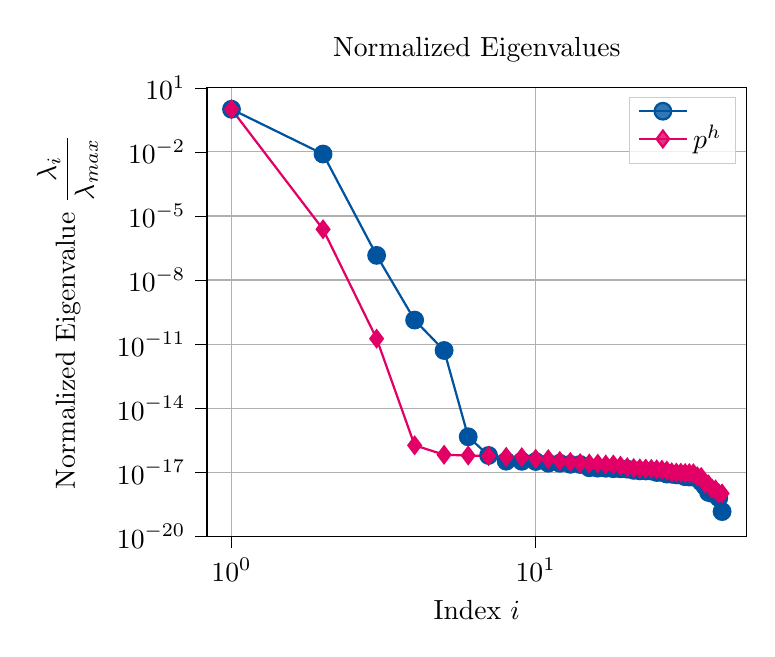
\begin{tikzpicture}

\definecolor{color0}{rgb}{0,0.329411764705882,0.623529411764706}
\definecolor{color1}{rgb}{0.890196078431372,0,0.4}

\begin{axis}[
legend cell align={left},
legend style={fill opacity=0.8, draw opacity=1, text opacity=1, draw=white!80!black},
log basis x={10},
log basis y={10},
tick align=outside,
tick pos=left,
title={Normalized Eigenvalues},
x grid style={white!69.0196078431373!black},
xlabel={Index \(\displaystyle i\)},
xmajorgrids,
xmin=0.830540485032707, xmax=49.3654442364545,
xmode=log,
xtick style={color=black},
xtick={0.01,0.1,1,10,100,1000},
xticklabels={
  \(\displaystyle 10^{-2}\),
  \(\displaystyle 10^{-1}\),
  \(\displaystyle 10^{0}\),
  \(\displaystyle 10^{1}\),
  \(\displaystyle 10^{2}\),
  \(\displaystyle 10^{3}\)
},
y grid style={white!69.0196078431373!black},
ylabel={Normalized Eigenvalue \(\displaystyle \frac{\lambda_i}{\lambda_{\text{max}}}\)},
ymajorgrids,
ymin=1e-20, ymax=10,
ymode=log,
ytick style={color=black},
ytick={1e-23,1e-20,1e-17,1e-14,1e-11,1e-08,1e-05,0.01,10,10000},
yticklabels={
  \(\displaystyle 10^{-23}\),
  \(\displaystyle 10^{-20}\),
  \(\displaystyle 10^{-17}\),
  \(\displaystyle 10^{-14}\),
  \(\displaystyle 10^{-11}\),
  \(\displaystyle 10^{-8}\),
  \(\displaystyle 10^{-5}\),
  \(\displaystyle 10^{-2}\),
  \(\displaystyle 10^{1}\),
  \(\displaystyle 10^{4}\)
}
]
\addplot [thick, color0, mark=*, mark size=3, mark options={solid}]
table {%
1 1
2 0.00794975858415845
3 1.42582257382325e-07
4 1.32791974403868e-10
5 5.00366283890635e-12
6 4.54114155240754e-16
7 6.04573529497411e-17
8 3.26201133022688e-17
9 3.22574638852698e-17
10 3.15358446366046e-17
11 2.62454621731955e-17
12 2.60840954654917e-17
13 2.33242093571454e-17
14 2.28813585566599e-17
15 1.60218882337199e-17
16 1.54306862706516e-17
17 1.52807821353466e-17
18 1.44864745846082e-17
19 1.43851705211444e-17
20 1.38677194525787e-17
21 1.21734236816605e-17
22 1.14897279038485e-17
23 1.13956935268721e-17
24 1.12564920102658e-17
25 9.63808041350083e-18
26 9.58979066065725e-18
27 8.13046505587439e-18
28 8.00740202533402e-18
29 7.46188080562777e-18
30 7.26718042554605e-18
31 6.11314351785897e-18
32 5.93273799548898e-18
33 5.84970067761768e-18
34 5.29939613242502e-18
35 3.47549460184894e-18
36 2.1905261247255e-18
37 1.12228744856004e-18
38 1.01406198292573e-18
39 9.59373162820783e-19
40 6.26226288149959e-19
41 1.42523827201686e-19
};
\addlegendentry{$\trialVelocityHomDiscrete$}
\addplot [thick, color1, mark=diamond*, mark size=3, mark options={solid}]
table {%
1 1
2 2.37328846603967e-06
3 1.78817929292869e-11
4 1.81154657334976e-16
5 6.51678466039161e-17
6 6.02235881107004e-17
7 5.69247083103718e-17
8 5.20065737906182e-17
9 5.01348143603465e-17
10 4.20958043774671e-17
11 4.07622974109276e-17
12 3.32697934377648e-17
13 2.98511733192585e-17
14 2.64421964531683e-17
15 2.52583071694472e-17
16 2.48386648445979e-17
17 2.27569426656641e-17
18 2.27247846357554e-17
19 1.99821382141988e-17
20 1.70491132142761e-17
21 1.54624364513944e-17
22 1.49112670601225e-17
23 1.45406520529215e-17
24 1.40935012359226e-17
25 1.35426769923973e-17
26 1.2976308799412e-17
27 1.18179500955933e-17
28 9.80114361457536e-18
29 9.51423374282225e-18
30 9.36239599182889e-18
31 9.08584610553105e-18
32 8.96571848518543e-18
33 8.78366822577326e-18
34 6.40001828288954e-18
35 5.93546015704658e-18
36 2.97856912325833e-18
37 2.64216217074413e-18
38 1.67829393129063e-18
39 1.53977850304594e-18
40 1.02797999983454e-18
41 1.00473640799576e-18
};
\addlegendentry{$p^h$}
\end{axis}

\end{tikzpicture}

        }
    }
    \subcaptionbox{Maximum interpolation error during the \gls{eim}.\label{fig:artery-likeEIMErrors}}{
        \resizebox{0.44\textwidth}{!}{
        % This file was created by tikzplotlib v0.9.8.
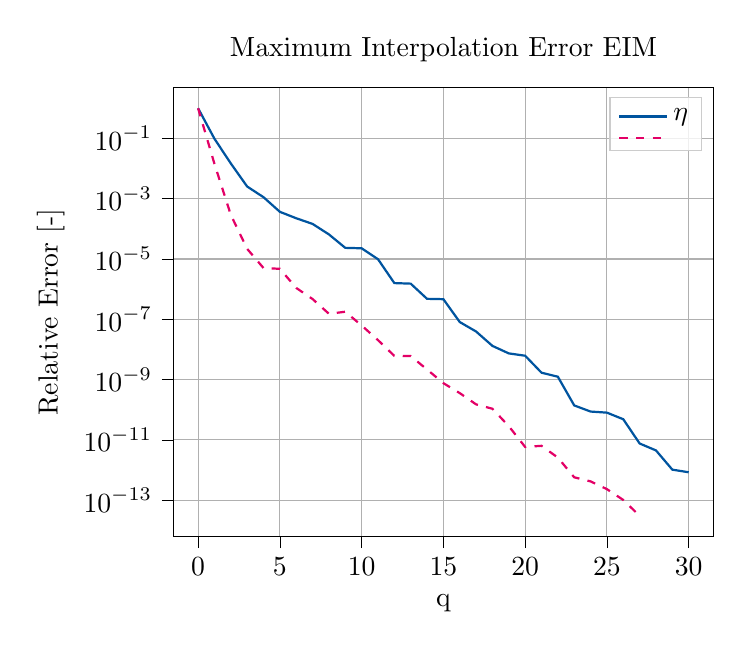
\begin{tikzpicture}

%\definecolor{color0}{rgb}{0.12156862745098,0.466666666666667,0.705882352941177}
%\definecolor{color1}{rgb}{1,0.498039215686275,0.0549019607843137}
\definecolor{color0}{rgb}{0,0.329411764705882,0.623529411764706}
\definecolor{color1}{rgb}{0.890196078431372,0,0.4}

\begin{axis}[
legend cell align={left},
legend style={fill opacity=0.8, draw opacity=1, text opacity=1, draw=white!80!black},
log basis y={10},
tick align=outside,
tick pos=left,
title={Maximum Interpolation Error EIM},
x grid style={white!69.0196078431373!black},
xlabel={q},
xmajorgrids,
xmin=-1.5, xmax=31.5,
xtick style={color=black},
xtick={-5,0,5,10,15,20,25,30,35},
xticklabels={
  \(\displaystyle -5\),
  \(\displaystyle 0\),
  \(\displaystyle 5\),
  \(\displaystyle 10\),
  \(\displaystyle 15\),
  \(\displaystyle 20\),
  \(\displaystyle 25\),
  \(\displaystyle 30\),
  \(\displaystyle 35\)
},
y grid style={white!69.0196078431373!black},
ylabel={Relative Error [-]},
ymajorgrids,
ymin=6.32307985340846e-15, ymax=4.74401718941179,
ymode=log,
ytick style={color=black},
ytick={1e-17,1e-15,1e-13,1e-11,1e-09,1e-07,1e-05,0.001,0.1,10,1000},
yticklabels={
  \(\displaystyle 10^{-17}\),
  \(\displaystyle 10^{-15}\),
  \(\displaystyle 10^{-13}\),
  \(\displaystyle 10^{-11}\),
  \(\displaystyle 10^{-9}\),
  \(\displaystyle 10^{-7}\),
  \(\displaystyle 10^{-5}\),
  \(\displaystyle 10^{-3}\),
  \(\displaystyle 10^{-1}\),
  \(\displaystyle 10^{1}\),
  \(\displaystyle 10^{3}\)
}
]
\addplot [thick, color0]
table {%
0 1
1 0.0973104687076621
2 0.0147633179066779
3 0.00252896805406514
4 0.00111793965375263
5 0.000366212967264887
6 0.000223970653068922
7 0.000145396874338459
8 6.52046804767942e-05
9 2.33321752580709e-05
10 2.26000046016262e-05
11 9.83915149206451e-06
12 1.58107750750885e-06
13 1.51597207604619e-06
14 4.75253511891816e-07
15 4.62299885501037e-07
16 8.06828170742323e-08
17 3.91006462079267e-08
18 1.30274119864675e-08
19 7.34041907118899e-09
20 6.15222072195395e-09
21 1.68400090499216e-09
22 1.23647681875085e-09
23 1.37973957655849e-10
24 8.64119044176524e-11
25 7.94881273897501e-11
26 4.80229695295645e-11
27 7.53378014734756e-12
28 4.43333366049816e-12
29 1.02026522151379e-12
30 8.36384533060246e-13
};
\addlegendentry{$\eta$}
\addplot [thick, color1, dashed]
table {%
0 1
1 0.0142591882104696
2 0.000290151916957558
3 2.16083662357261e-05
4 4.98689894693042e-06
5 4.70515968704204e-06
6 1.0922818762808e-06
7 4.67179954054551e-07
8 1.51464068402887e-07
9 1.77303957247854e-07
10 6.20554933265058e-08
11 2.02888056647836e-08
12 6.08014447268978e-09
13 5.99435297181841e-09
14 2.15022814619033e-09
15 7.55822336917672e-10
16 3.5378735937984e-10
17 1.49573256052504e-10
18 1.06992880868169e-10
19 2.82133502676071e-11
20 5.78225645869476e-12
21 6.30593569710007e-12
22 2.5585361244864e-12
23 5.685980701701e-13
24 4.16003286360201e-13
25 2.3040791442305e-13
26 1.00534473647095e-13
27 2.99967995145931e-14
};
\addlegendentry{$\tMomPlain$}
\end{axis}

\end{tikzpicture}

        }
    }
    \caption{Artery-like test case: results from the construction of the \gls{rom}.}
    \label{fig:artery-likeOffline}
\end{figure}
\par
\begin{figure}
    \captionsetup[sub]{position=bottom}
    \centering
    \Large
    \subcaptionbox{Velocity.}{
        \resizebox{0.44\textwidth}{!}{
        % This file was created by tikzplotlib v0.9.8.
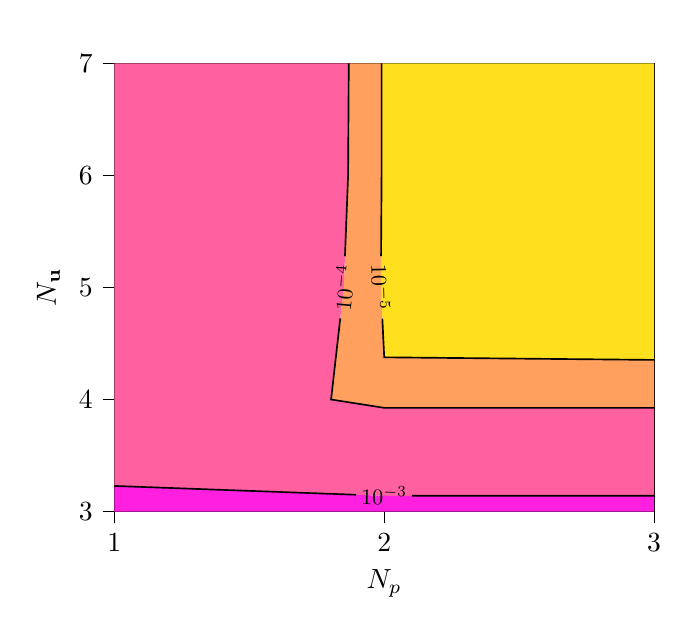
\begin{tikzpicture}

\definecolor{color0}{rgb}{1,0.87843137254902,0.12156862745098}
\definecolor{color1}{rgb}{1,0.627450980392157,0.372549019607843}
\definecolor{color2}{rgb}{1,0.376470588235294,0.623529411764706}
\definecolor{color3}{rgb}{1,0.125490196078431,0.874509803921569}

\begin{axis}[
tick align=outside,
tick pos=left,
%title={Relative Error in Velocity \(\displaystyle \mathbf{u}\) - Max},
title={$\relErrorVelocity$},
x grid style={white!69.0196078431373!black},
xlabel={\(\displaystyle N_p\)},
xmin=1, xmax=3,
xtick style={color=black},
xtick={1,2,3},
xticklabels={\(\displaystyle 1\),\(\displaystyle 2\),\(\displaystyle 3\)},
y grid style={white!69.0196078431373!black},
ylabel={\(\displaystyle N_{\mathbf{u}}\)},
ymin=3, ymax=7,
ytick style={color=black},
ytick={3,4,5,6,7},
yticklabels={
  \(\displaystyle 3\),
  \(\displaystyle 4\),
  \(\displaystyle 5\),
  \(\displaystyle 6\),
  \(\displaystyle 7\)
}
]
\addplot [draw=none, fill=color0]
table{%
x  y
2 4.37650891394412
3 4.35330770412385
3 5
3 6
3 7
2 7
1.99040991259345 7
1.9903127173998 6
1.98760845108052 5
2 4.37650891394412
};
\addplot [draw=none, fill=color1]
table{%
x  y
2 3.92579367910137
3 3.92540471448223
3 4
3 4.35330770412385
2 4.37650891394412
1.98760845108052 5
1.9903127173998 6
1.99040991259345 7
1.86869012295147 7
1.86619036626405 6
1.85013870710813 5
1.80309130655496 4
2 3.92579367910137
};
\addplot [draw=none, fill=color2]
table{%
x  y
2 3.14101234840689
3 3.14081265825156
3 3.92540471448223
2 3.92579367910137
1.80309130655496 4
1.85013870710813 5
1.86619036626405 6
1.86869012295147 7
1 7
1 6
1 5
1 4
1 3.22895886838152
2 3.14101234840689
};
\addplot [draw=none, fill=color3]
table{%
x  y
2 3
3 3
3 3.14081265825156
2 3.14101234840689
1 3.22895886838152
1 3
2 3
};
\path [draw=black, semithick]
(axis cs:3,4.35330770412385)
--(axis cs:2,4.37650891394412)
--(axis cs:1.99313704618645,4.72182414084339);

\path [draw=black, semithick]
(axis cs:1.98836176234379,5.27856400751013)
--(axis cs:1.9903127173998,6)
--(axis cs:1.99040991259345,7);

\path [draw=black, semithick]
(axis cs:3,3.92540471448223)
--(axis cs:2,3.92579367910137)
--(axis cs:1.80309130655496,4)
--(axis cs:1.83713590577805,4.72362338456115);

\path [draw=black, semithick]
(axis cs:1.85460609537104,5.27831317744237)
--(axis cs:1.86619036626405,6)
--(axis cs:1.86869012295147,7);

\path [draw=black, semithick]
(axis cs:3,3.14081265825156)
--(axis cs:2.10379029115697,3.14099162250753);

\path [draw=black, semithick]
(axis cs:1.89626538289669,3.15013544698203)
--(axis cs:1,3.22895886838152);

\draw (axis cs:1.98760845108052,5) node[
  scale=0.8,
  text=black,
  rotate=271.3
]{$10^{-5}$};
\draw (axis cs:1.85013870710813,5) node[
  scale=0.8,
  text=black,
  rotate=85.2
]{$10^{-4}$};
\draw (axis cs:2,3.14101234840689) node[
  scale=0.8,
  text=black,
  rotate=359.1
]{$10^{-3}$};
\end{axis}

\end{tikzpicture}
}
    }
    \subcaptionbox{Pressure.}{
        \resizebox{0.44\textwidth}{!}{
        % This file was created by tikzplotlib v0.9.8.
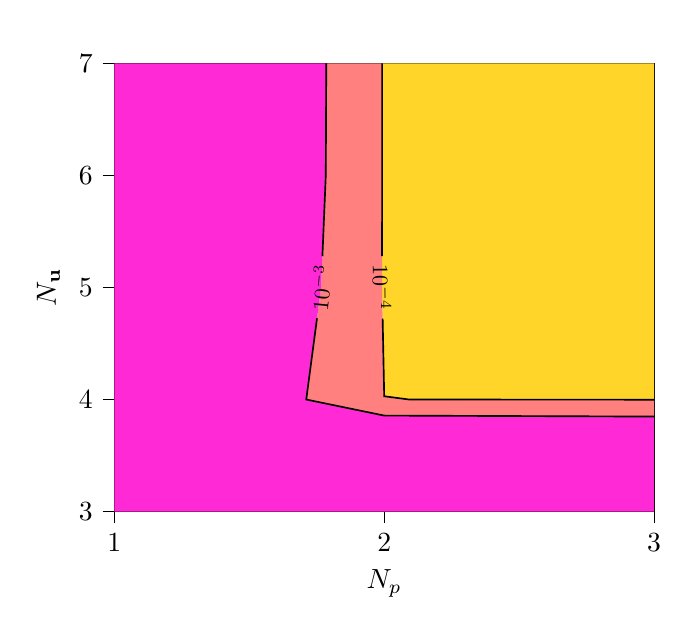
\begin{tikzpicture}

\definecolor{color0}{rgb}{1,0.835294117647059,0.164705882352941}
\definecolor{color1}{rgb}{1,0.501960784313725,0.498039215686275}
\definecolor{color2}{rgb}{1,0.164705882352941,0.835294117647059}

\begin{axis}[
tick align=outside,
tick pos=left,
%title={Relative Error in Pressure \(\displaystyle p\) - Max},
title={$\relErrorPressure$},
x grid style={white!69.0196078431373!black},
xlabel={\(\displaystyle N_p\)},
xmin=1, xmax=3,
xtick style={color=black},
xtick={1,2,3},
xticklabels={\(\displaystyle 1\),\(\displaystyle 2\),\(\displaystyle 3\)},
y grid style={white!69.0196078431373!black},
ylabel={\(\displaystyle N_{\mathbf{u}}\)},
ymin=3, ymax=7,
ytick style={color=black},
ytick={3,4,5,6,7},
yticklabels={
  \(\displaystyle 3\),
  \(\displaystyle 4\),
  \(\displaystyle 5\),
  \(\displaystyle 6\),
  \(\displaystyle 7\)
}
]
\addplot [draw=none, fill=color0]
table{%
x  y
3 3.99841272096808
3 4
3 5
3 6
3 7
2 7
1.99231388686608 7
1.9923086500537 6
1.99186016592534 5
2 4.02906689026844
2.0929081054864 4
3 3.99841272096808
};
\addplot [draw=none, fill=color1]
table{%
x  y
2 3.85666988114318
3 3.84783564712328
3 3.99841272096808
2.0929081054864 4
2 4.02906689026844
1.99186016592534 5
1.9923086500537 6
1.99231388686608 7
1.78528526361933 7
1.78346767600251 6
1.76616198020346 5
1.71107969290604 4
2 3.85666988114318
};
\addplot [draw=none, fill=color2]
table{%
x  y
2 3
3 3
3 3.84783564712328
2 3.85666988114318
1.71107969290604 4
1.76616198020346 5
1.78346767600251 6
1.78528526361933 7
1 7
1 6
1 5
1 4
1 3
2 3
};
\path [draw=black, semithick]
(axis cs:3,3.99841272096808)
--(axis cs:2.0929081054864,4)
--(axis cs:2,4.02906689026844)
--(axis cs:1.99419498249751,4.72149914921187);

\path [draw=black, semithick]
(axis cs:1.99198510066168,5.278571143184)
--(axis cs:1.9923086500537,6)
--(axis cs:1.99231388686608,7);

\path [draw=black, semithick]
(axis cs:3,3.84783564712328)
--(axis cs:2,3.85666988114318)
--(axis cs:1.71107969290604,4)
--(axis cs:1.75098262156661,4.72442395946829);

\path [draw=black, semithick]
(axis cs:1.77097765920204,5.27827133069329)
--(axis cs:1.78346767600251,6)
--(axis cs:1.78528526361933,7);

\draw (axis cs:1.99186016592534,5) node[
  scale=0.8,
  text=black,
  rotate=270.6
]{$10^{-4}$};
\draw (axis cs:1.76616198020346,5) node[
  scale=0.8,
  text=black,
  rotate=84.5
]{$10^{-3}$};
\end{axis}

\end{tikzpicture}
}
    }
    \caption{Artery-like test case: maximum relative error of the \gls{rom} over all testing samples.}
    \label{fig:artery-likeRelativeErrorMax}
\end{figure}
\par
Next, we present the results from the performance analysis. The \gls{rom} has been evaluated on a single core, whereas we have used 240 cores to compute the \gls{fom}. The measured speed up --- the average and the maximum over all the testing samples --- is shown in \Cref{fig:artery-likePerformance}. The results are, to some extent, counter-intuitive. First, one can observe that the speed up is mainly governed by $\nBasisVelocityROM$ and roughly constant for  $\nBasisPressureROM$. Second, the speed up does not change monotonically with increasing $\nBasisVelocityROM$ but has a local maximum at $\nBasisVelocityROM=5$. Analyzing the evaluation of the \gls{rom} in more detail has revealed that this pattern originates from the number of iterations needed to solve the non-linear reduced system. In particular, the value for $\nBasisVelocityROM$ influences the number of non-linear iterations and, in some cases, slows down the solution process. Nevertheless, the order of magnitude of the observed speed up, ranging from 25,000 to 60,000, is still compelling and even much more significant than in the previous test case.
\begin{figure}
    \captionsetup[sub]{position=bottom}
    \centering
    \Large
    \subcaptionbox{Average speed up over all testing samples.}{
        \resizebox{0.44\textwidth}{!}{
        % This file was created by tikzplotlib v0.9.8.
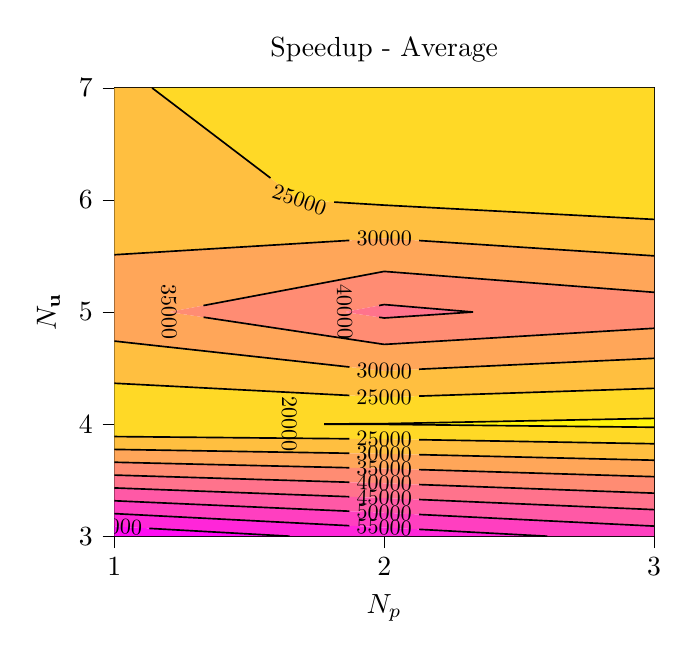
\begin{tikzpicture}

\definecolor{color0}{rgb}{1,0.952941176470588,0.0470588235294118}
\definecolor{color1}{rgb}{1,0.850980392156863,0.149019607843137}
\definecolor{color2}{rgb}{1,0.749019607843137,0.250980392156863}
\definecolor{color3}{rgb}{1,0.650980392156863,0.349019607843137}
\definecolor{color4}{rgb}{1,0.549019607843137,0.450980392156863}
\definecolor{color5}{rgb}{1,0.450980392156863,0.549019607843137}
\definecolor{color6}{rgb}{1,0.349019607843137,0.650980392156863}
\definecolor{color7}{rgb}{1,0.247058823529412,0.752941176470588}
\definecolor{color8}{rgb}{1,0.149019607843137,0.850980392156863}
\definecolor{color9}{rgb}{1,0.0470588235294118,0.952941176470588}

\begin{axis}[
tick align=outside,
tick pos=left,
title={Speedup - Average},
x grid style={white!69.0196078431373!black},
xlabel={\(\displaystyle N_p\)},
xmin=1, xmax=3,
xtick style={color=black},
xtick={1,2,3},
xticklabels={\(\displaystyle 1\),\(\displaystyle 2\),\(\displaystyle 3\)},
y grid style={white!69.0196078431373!black},
ylabel={\(\displaystyle N_{\mathbf{u}}\)},
ymin=3, ymax=7,
ytick style={color=black},
ytick={3,4,5,6,7},
yticklabels={
  \(\displaystyle 3\),
  \(\displaystyle 4\),
  \(\displaystyle 5\),
  \(\displaystyle 6\),
  \(\displaystyle 7\)
}
]
\addplot [draw=none, fill=color0]
table{%
x  y
2 3.99776029877739
3 3.97186061500088
3 4
3 4.05129247948725
2 4.00401665310977
1.64783776122399 4
2 3.99776029877739
};
\addplot [draw=none, fill=color1]
table{%
x  y
2 3.86632751738316
3 3.82489079580478
3 3.97186061500088
2 3.99776029877739
1.64783776122399 4
2 4.00401665310977
3 4.05129247948725
3 4.31918911036938
2 4.23972661512697
1 4.36447852644752
1 4
1 3.88899847255399
2 3.86632751738316
};
\addplot [draw=none, fill=color1]
table{%
x  y
2 5.95377752187074
3 5.82647002301902
3 6
3 7
2 7
1.13955470147603 7
1.68538959041588 6
2 5.95377752187074
};
\addplot [draw=none, fill=color2]
table{%
x  y
2 3.73489473598894
3 3.67792097660869
3 3.82489079580478
2 3.86632751738316
1 3.88899847255399
1 3.77440465802077
2 3.73489473598894
};
\addplot [draw=none, fill=color2]
table{%
x  y
2 4.23972661512697
3 4.31918911036938
3 4.58708574125151
2 4.47543657714418
1 4.74075248971692
1 4.36447852644752
2 4.23972661512697
};
\addplot [draw=none, fill=color2]
table{%
x  y
2 5.65807486026756
3 5.50125704822069
3 5.82647002301902
2 5.95377752187074
1.68538959041588 6
1.13955470147603 7
1 7
1 6
1 5.51094647432634
2 5.65807486026756
};
\addplot [draw=none, fill=color3]
table{%
x  y
2 3.60346195459471
3 3.5309511574126
3 3.67792097660869
2 3.73489473598894
1 3.77440465802077
1 3.65981084348756
2 3.60346195459471
};
\addplot [draw=none, fill=color3]
table{%
x  y
2 4.47543657714418
3 4.58708574125151
3 4.85498237213365
2 4.71114653916139
1.20242039825908 5
2 5.36237219866437
3 5.17604407342235
3 5.50125704822069
2 5.65807486026756
1 5.51094647432634
1 5
1 4.74075248971692
2 4.47543657714418
};
\addplot [draw=none, fill=color4]
table{%
x  y
2 3.47202917320049
3 3.38398133821651
3 3.5309511574126
2 3.60346195459471
1 3.65981084348756
1 3.54521702895434
2 3.47202917320049
};
\addplot [draw=none, fill=color4]
table{%
x  y
2 4.71114653916139
3 4.85498237213365
3 5
3 5.17604407342235
2 5.36237219866437
1.20242039825908 5
2 4.71114653916139
1.85326064468108 5
2 5.06666953706118
2.3295534889383 5
2 4.94685650117859
1.85326064468108 5
};
\addplot [draw=none, fill=color5]
table{%
x  y
2 3.34059639180626
3 3.23701151902041
3 3.38398133821651
2 3.47202917320049
1 3.54521702895434
1 3.43062321442112
2 3.34059639180626
};
\addplot [draw=none, fill=color5]
table{%
x  y
2 4.94685650117859
2.3295534889383 5
2 5.06666953706118
1.85326064468108 5
2 4.94685650117859
};
\addplot [draw=none, fill=color6]
table{%
x  y
2 3.20916361041203
3 3.09004169982432
3 3.23701151902041
2 3.34059639180626
1 3.43062321442112
1 3.3160293998879
2 3.20916361041203
};
\addplot [draw=none, fill=color7]
table{%
x  y
2 3.07773082901781
2.60424735056556 3
3 3
3 3.09004169982432
2 3.20916361041203
1 3.3160293998879
1 3.20143558535469
2 3.07773082901781
};
\addplot [draw=none, fill=color8]
table{%
x  y
2 3
2.60424735056556 3
2 3.07773082901781
1 3.20143558535469
1 3.08684177082147
1.64970439596316 3
2 3
};
\addplot [draw=none, fill=color9]
table{%
x  y
1 3.08684177082147
1 3
1.64970439596316 3
1 3.08684177082147
};
\path [draw=black, semithick]
(axis cs:3,3.97186061500088)
--(axis cs:2,3.99776029877739)
--(axis cs:1.77726149904818,3.99917688362941);

\path [draw=black, semithick]
(axis cs:1.77726069380053,4.00147615776869)
--(axis cs:2,4.00401665310977)
--(axis cs:3,4.05129247948725);

\path [draw=black, semithick]
(axis cs:3,3.82489079580478)
--(axis cs:2.12940867994302,3.86096524594254);

\path [draw=black, semithick]
(axis cs:1.87058051564284,3.86926158071125)
--(axis cs:1,3.88899847255399);

\path [draw=black, semithick]
(axis cs:1,4.36447852644752)
--(axis cs:1.87071547689406,4.2558551064886);

\path [draw=black, semithick]
(axis cs:2.12936741661236,4.25000647285406)
--(axis cs:3,4.31918911036938);

\path [draw=black, semithick]
(axis cs:3,5.82647002301902)
--(axis cs:2,5.95377752187074)
--(axis cs:1.81462022259509,5.98101346971504);

\path [draw=black, semithick]
(axis cs:1.57849420274952,6.1958383200348)
--(axis cs:1.13955470147603,7);

\path [draw=black, semithick]
(axis cs:3,3.67792097660869)
--(axis cs:2.1293949518265,3.72752261913855);

\path [draw=black, semithick]
(axis cs:1.87058991946085,3.74000771818117)
--(axis cs:1,3.77440465802077);

\path [draw=black, semithick]
(axis cs:1,4.74075248971692)
--(axis cs:1.87120364443596,4.5096082997567);

\path [draw=black, semithick]
(axis cs:2.12931226725914,4.48987418369249)
--(axis cs:3,4.58708574125151);

\path [draw=black, semithick]
(axis cs:3,5.50125704822069)
--(axis cs:2.12920375458042,5.63781341016601);

\path [draw=black, semithick]
(axis cs:1.87076991649158,5.63906144666591)
--(axis cs:1,5.51094647432634);

\path [draw=black, semithick]
(axis cs:3,3.5309511574126)
--(axis cs:2.12937689557672,3.5940807327595);

\path [draw=black, semithick]
(axis cs:1.87060441248816,3.61075325217864)
--(axis cs:1,3.65981084348756);

\path [draw=black, semithick]
(axis cs:3,5.17604407342235)
--(axis cs:2,5.36237219866437)
--(axis cs:1.33002909148532,5.05797771486651);

\path [draw=black, semithick]
(axis cs:1.33068211116719,4.95354841123603)
--(axis cs:2,4.71114653916139)
--(axis cs:3,4.85498237213365);

\path [draw=black, semithick]
(axis cs:3,3.38398133821651)
--(axis cs:2.12935451663035,3.46063978806578);

\path [draw=black, semithick]
(axis cs:1.87062398959549,3.48149792598798)
--(axis cs:1,3.54521702895434);

\path [draw=black, semithick]
(axis cs:1.98152235758919,4.95354841123603)
--(axis cs:2,4.94685650117859)
--(axis cs:2.3295534889383,5)
--(axis cs:2,5.06666953706118)
--(axis cs:1.98086933790731,5.05797771486651);

\path [draw=black, semithick]
(axis cs:3,3.23701151902041)
--(axis cs:2.12932782172,3.32719998584572);

\path [draw=black, semithick]
(axis cs:1.87064864385909,3.35224148340055)
--(axis cs:1,3.43062321442112);

\path [draw=black, semithick]
(axis cs:3,3.09004169982432)
--(axis cs:2.12929681886861,3.19376152631549);

\path [draw=black, semithick]
(axis cs:1.87067836656755,3.2229836688651)
--(axis cs:1,3.3160293998879);

\path [draw=black, semithick]
(axis cs:2.60424735056556,3)
--(axis cs:2.12927570066499,3.06110070664302);

\path [draw=black, semithick]
(axis cs:1.87071314723031,3.09372422763725)
--(axis cs:1,3.20143558535469);

\path [draw=black, semithick]
(axis cs:1.64970439596316,3)
--(axis cs:1.12926390778472,3.06956390303255);

\draw (axis cs:1.64783776122399,4) node[
  scale=0.8,
  text=black,
  rotate=270.1
]{20000};
\draw (axis cs:2,3.86632751738316) node[
  scale=0.8,
  text=black,
  rotate=359.3
]{25000};
\draw (axis cs:2,4.23972661512697) node[
  scale=0.8,
  text=black,
  rotate=359.5
]{25000};
\draw (axis cs:1.68538959041588,6) node[
  scale=0.8,
  text=black,
  rotate=341.3
]{25000};
\draw (axis cs:2,3.73489473598894) node[
  scale=0.8,
  text=black,
  rotate=359.0
]{30000};
\draw (axis cs:2,4.47543657714418) node[
  scale=0.8,
  text=black,
  rotate=358.4
]{30000};
\draw (axis cs:2,5.65807486026756) node[
  scale=0.8,
  text=black,
  rotate=359.9
]{30000};
\draw (axis cs:2,3.60346195459471) node[
  scale=0.8,
  text=black,
  rotate=358.6
]{35000};
\draw (axis cs:1.20242039825908,5) node[
  scale=0.8,
  text=black,
  rotate=271.0
]{35000};
\draw (axis cs:2,3.47202917320049) node[
  scale=0.8,
  text=black,
  rotate=358.3
]{40000};
\draw (axis cs:1.85326064468108,5) node[
  scale=0.8,
  text=black,
  rotate=271.0
]{40000};
\draw (axis cs:2,3.34059639180626) node[
  scale=0.8,
  text=black,
  rotate=357.9
]{45000};
\draw (axis cs:2,3.20916361041203) node[
  scale=0.8,
  text=black,
  rotate=357.6
]{50000};
\draw (axis cs:2,3.07773082901781) node[
  scale=0.8,
  text=black,
  rotate=357.3
]{55000};
\draw (axis cs:1,3.08684177082147) node[
  scale=0.8,
  text=black,
  rotate=357.1
]{60000};
\end{axis}

\end{tikzpicture}
}
    }
    \subcaptionbox{Maximum speed up over all testing samples.}{
        \resizebox{0.44\textwidth}{!}{
        % This file was created by tikzplotlib v0.9.8.
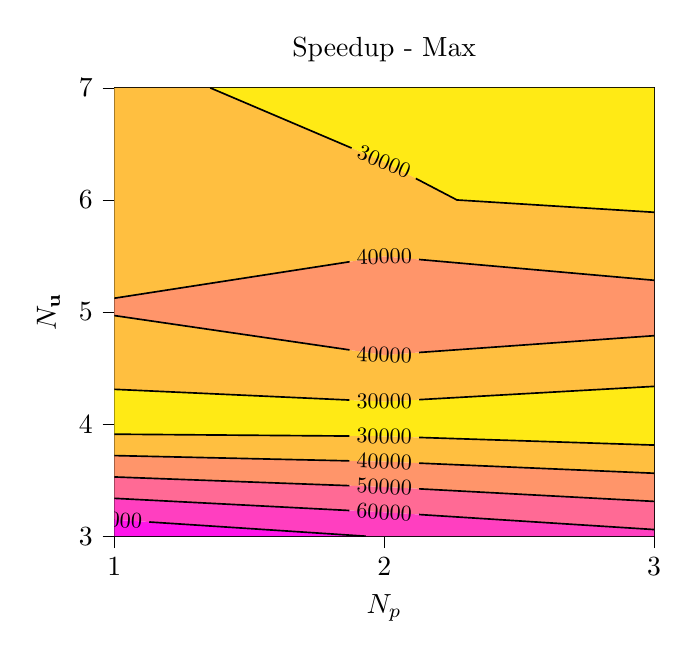
\begin{tikzpicture}

\definecolor{color0}{rgb}{1,0.917647058823529,0.0823529411764706}
\definecolor{color1}{rgb}{1,0.749019607843137,0.250980392156863}
\definecolor{color2}{rgb}{1,0.584313725490196,0.415686274509804}
\definecolor{color3}{rgb}{1,0.415686274509804,0.584313725490196}
\definecolor{color4}{rgb}{1,0.247058823529412,0.752941176470588}
\definecolor{color5}{rgb}{1,0.0823529411764706,0.917647058823529}

\begin{axis}[
tick align=outside,
tick pos=left,
title={Speedup - Max},
x grid style={white!69.0196078431373!black},
xlabel={\(\displaystyle N_p\)},
xmin=1, xmax=3,
xtick style={color=black},
xtick={1,2,3},
xticklabels={\(\displaystyle 1\),\(\displaystyle 2\),\(\displaystyle 3\)},
y grid style={white!69.0196078431373!black},
ylabel={\(\displaystyle N_{\mathbf{u}}\)},
ymin=3, ymax=7,
ytick style={color=black},
ytick={3,4,5,6,7},
yticklabels={
  \(\displaystyle 3\),
  \(\displaystyle 4\),
  \(\displaystyle 5\),
  \(\displaystyle 6\),
  \(\displaystyle 7\)
}
]
\addplot [draw=none, fill=color0]
table{%
x  y
2 3.89113969366561
3 3.81295761379902
3 4
3 4.33664393194555
2 4.20059943824401
1 4.31046717020061
1 4
1 3.91000519290614
2 3.89113969366561
};
\addplot [draw=none, fill=color0]
table{%
x  y
3 5.8901285826523
3 6
3 7
2 7
1.35534430289395 7
2 6.33923453361608
2.26948248989546 6
3 5.8901285826523
};
\addplot [draw=none, fill=color1]
table{%
x  y
2 3.66515692779255
3 3.56174755756104
3 3.81295761379902
2 3.89113969366561
1 3.91000519290614
1 3.71929144543007
2 3.66515692779255
};
\addplot [draw=none, fill=color1]
table{%
x  y
2 4.20059943824401
3 4.33664393194555
3 4.78877856727545
2 4.61702317811216
1 4.96839799320352
1 4.31046717020061
2 4.20059943824401
};
\addplot [draw=none, fill=color1]
table{%
x  y
2 5.49635319629926
3 5.28342883044444
3 5.8901285826523
2.26948248989546 6
2 6.33923453361608
1.35534430289395 7
1 7
1 6
1 5.12326574274158
2 5.49635319629926
};
\addplot [draw=none, fill=color2]
table{%
x  y
2 3.4391741619195
3 3.31053750132306
3 3.56174755756104
2 3.66515692779255
1 3.71929144543007
1 3.52857769795399
2 3.4391741619195
};
\addplot [draw=none, fill=color2]
table{%
x  y
2 4.61702317811216
3 4.78877856727545
3 5
3 5.28342883044444
2 5.49635319629926
1 5.12326574274158
1 5
1 4.96839799320352
2 4.61702317811216
};
\addplot [draw=none, fill=color3]
table{%
x  y
2 3.21319139604645
3 3.05932744508508
3 3.31053750132306
2 3.4391741619195
1 3.52857769795399
1 3.33786395047791
2 3.21319139604645
};
\addplot [draw=none, fill=color4]
table{%
x  y
2 3
3 3
3 3.05932744508508
2 3.21319139604645
1 3.33786395047791
1 3.14715020300184
1.93165335182826 3
2 3
};
\addplot [draw=none, fill=color5]
table{%
x  y
1 3.14715020300184
1 3
1.93165335182826 3
1 3.14715020300184
};
\path [draw=black, semithick]
(axis cs:3,3.81295761379902)
--(axis cs:2.12936922751048,3.8810253383881);

\path [draw=black, semithick]
(axis cs:1.87057909585802,3.89358128363441)
--(axis cs:1,3.91000519290614);

\path [draw=black, semithick]
(axis cs:1,4.31046717020061)
--(axis cs:1.87068419689434,4.21480707223737);

\path [draw=black, semithick]
(axis cs:2.12925816089073,4.21818429929918)
--(axis cs:3,4.33664393194555);

\path [draw=black, semithick]
(axis cs:3,5.8901285826523)
--(axis cs:2.26948248989546,6)
--(axis cs:2.11717612375158,6.19172889157148);

\path [draw=black, semithick]
(axis cs:1.87909257266006,6.46316340444465)
--(axis cs:1.35534430289395,7);

\path [draw=black, semithick]
(axis cs:3,3.56174755756104)
--(axis cs:2.12932814733133,3.65178318552381);

\path [draw=black, semithick]
(axis cs:1.87060221616005,3.67216181440409)
--(axis cs:1,3.71929144543007);

\path [draw=black, semithick]
(axis cs:1,4.96839799320352)
--(axis cs:1.87167093357662,4.66211478009752);

\path [draw=black, semithick]
(axis cs:2.12915991192253,4.63920708904871)
--(axis cs:3,4.78877856727545);

\path [draw=black, semithick]
(axis cs:3,5.28342883044444)
--(axis cs:2.12901874905936,5.46888196097241);

\path [draw=black, semithick]
(axis cs:1.87180845969371,5.44852654095875)
--(axis cs:1,5.12326574274158);

\path [draw=black, semithick]
(axis cs:3,3.31053750132306)
--(axis cs:2.12927571007098,3.42254456627974);

\path [draw=black, semithick]
(axis cs:1.87064764090286,3.45073872021719)
--(axis cs:1,3.52857769795399);

\path [draw=black, semithick]
(axis cs:3,3.05932744508508)
--(axis cs:2.12921195720541,3.19331033379938);

\path [draw=black, semithick]
(axis cs:1.87071529966112,3.22930964988661)
--(axis cs:1,3.33786395047791);

\path [draw=black, semithick]
(axis cs:1.93165335182826,3)
--(axis cs:1.12920058312662,3.12674358717447);

\draw (axis cs:2,3.89113969366561) node[
  scale=0.8,
  text=black,
  rotate=359.0
]{30000};
\draw (axis cs:2,4.20059943824401) node[
  scale=0.8,
  text=black,
  rotate=0.3
]{30000};
\draw (axis cs:2,6.33923453361608) node[
  scale=0.8,
  text=black,
  rotate=337.0
]{30000};
\draw (axis cs:2,3.66515692779255) node[
  scale=0.8,
  text=black,
  rotate=358.3
]{40000};
\draw (axis cs:2,4.61702317811216) node[
  scale=0.8,
  text=black,
  rotate=358.1
]{40000};
\draw (axis cs:2,5.49635319629926) node[
  scale=0.8,
  text=black,
  rotate=1.7
]{40000};
\draw (axis cs:2,3.4391741619195) node[
  scale=0.8,
  text=black,
  rotate=357.7
]{50000};
\draw (axis cs:2,3.21319139604645) node[
  scale=0.8,
  text=black,
  rotate=357.0
]{60000};
\draw (axis cs:1,3.14715020300184) node[
  scale=0.8,
  text=black,
  rotate=356.6
]{70000};
\end{axis}

\end{tikzpicture}
}
    }
    \caption{Artery-like test case: performance results.}
    \label{fig:artery-likePerformance}
\end{figure}
\par
So, also the results for this test case underline the advantages of the proposed approach in general and, specifically, its ability to handle problems defined in a four-dimensional space-time domain. 
